\documentclass[a4paper,twoside]{scrbook}
\usepackage{layout}
\usepackage{amsmath, amsthm}
\usepackage{amssymb, amsrefs}
\usepackage{stmaryrd}
\usepackage{graphicx}
\usepackage{setspace}
\usepackage{textcomp}
\usepackage{esvect}
\usepackage[letterpaper]{geometry}
\usepackage{arydshln}
\usepackage[all]{xy}
\usepackage{etex}

\usepackage[dvipsnames]{xcolor}  


\usepackage{epsfig}
\usepackage{latexsym}
\usepackage{amsthm}

\usepackage{mathrsfs}

\usepackage[colorlinks,citecolor=blue]{hyperref}

\usepackage[latin1]{inputenc}

\usepackage{tikz-cd}
\usetikzlibrary{graphs,graphs.standard}
\usepackage{pgfplots}
\usetikzlibrary{matrix,arrows,decorations.pathmorphing}
\usetikzlibrary{shapes.geometric}

\newtheorem{theorem}{Theorem}[section]
\newtheorem{lemma}[theorem]{Lemma}
\newtheorem{proposition}[theorem]{Proposition}
\newtheorem{prop}[theorem]{Proposition}
\newtheorem{corollary}[theorem]{Corollary}
\newtheorem{cor}[theorem]{Corollary}

\theoremstyle{definition}
\newtheorem{definition}[theorem]{Definition}
\newtheorem{defn}[theorem]{Definition}
\newtheorem{example}[theorem]{Example}
\newtheorem{problem}[equation]{Problem}
\newtheorem{remark}[theorem]{Remark}
\newtheorem{obs}[theorem]{Observation}



\theoremstyle{definition}
\numberwithin{equation}{section}


\DeclareGraphicsRule{.tif}{png}{.png}{`convert #1 `dirname
#1`/`basename #1 .tif`.png}
\tikzset{
    ncbar angle/.initial=90,
    ncbar/.style={
        to path=(\tikztostart)
        -- ($(\tikztostart)!#1!\pgfkeysvalueof{/tikz/ncbar angle}:(\tikztotarget)$)
        -- ($(\tikztotarget)!($(\tikztostart)!#1!\pgfkeysvalueof{/tikz/ncbar angle}:(\tikztotarget)$)!\pgfkeysvalueof{/tikz/ncbar angle}:(\tikztostart)$)
        -- (\tikztotarget)
    },
    ncbar/.default=0.5cm,
}

\tikzset{square left brace/.style={ncbar=0.5cm}}
\tikzset{square right brace/.style={ncbar=-0.5cm}}

\tikzset{round left paren/.style={ncbar=0.5cm,out=120,in=-120}}
\tikzset{round right paren/.style={ncbar=0.5cm,out=60,in=-60}}

\newcommand{\Q}{\textbf{Question:\ }}
\newcommand{\Sol}{\textbf{Solution:\ }}


\newcommand{\Fisg}{\text{\textnormal{Fisg}}}
\newcommand{\Iisg}{\text{\textnormal{Iisg}}}
\newcommand{\Pisg}{\text{\textnormal{Pisg}}}
\newcommand{\Tisg}{\text{\textnormal{Tisg}}}
\newcommand{\Dom}{\text{\textnormal{Dom}}}
\newcommand{\Img}{\text{\textnormal{Im}}}
\DeclareMathOperator{\id}{id}

\newcommand{\bcup}{\displaystyle\bigcup}
\newcommand{\bcap}{\displaystyle\bigcap}
\newcommand{\dsum}{\displaystyle\sum}
\newcommand{\dint}{\displaystyle\int}



\newcommand{\R}[1]{\mathbb{R}^{#1}}
\newcommand{\C}[1]{\mathbb{C}^{#1}}
\newcommand{\Z}[1]{\mathbb{Z}^{#1}}
\newcommand{\K}[1]{\mathbb{K}^{#1}}


\newcommand{\TCB}[1]{\textcolor{blue}{#1}}
\newcommand{\TCR}[1]{\textcolor{red}{#1}}
\newcommand{\TCO}[1]{\textcolor{orange}{#1}}
\newcommand{\TCG}[1]{\textcolor{ForestGreen}{#1}}



\DeclareMathOperator{\Endo}{Endo}
\DeclareMathOperator{\Aut}{Aut}

\DeclareMathOperator{\Hom}{Hom}
\DeclareMathOperator{\Obj}{Obj}

\DeclareMathOperator{\pleat}{\mathcal{P}\ell}



\def \PX {\mathfrak{W}G}

\def \Gph {\mathsf{Gph}}
\def \HoGph {\mathsf{HoGph}}
\def \into {\hookrightarrow}

\def \con {\underline{\phantom{w}}}
\definecolor{laura}{rgb}{.4, 0, .6}


%--------------------------------------------------------------------------------------------------------------------------------------------------

\begin{document}
\title{Finite Mathematics}
\subtitle{A Tour}
\author{Tien Chih}
\date{}
\frontmatter
\maketitle
\tableofcontents
\mainmatter
%

\chapter{Linear Functions}

\section*{Introduction}

        In this Chapter, we will introduce the notion of a \textbf{linear function}.  Linear functions are used to model a variety of situations, such as the the revenue generated by selling a product, conversion between units of measurement such as Fahrenheit to Celsius, distance traveled by an entity moving at a constant velocity, demand of a product relative to price and many more.  It is also a good introduction to the theory of functions more generally.


\section{What is a Linear Function?}

A linear function is a function whose inputs and outputs are real numbers, and \textit{the change in output per unit change increase in input is always the same.}  A linear function may always increase, or decrease, or stay the same, but the rate at which it does so will never change.

\begin{example}
Consider a function who takes on the following values:

$$\begin{array}{|c||c|c|c|c|c|}
\hline
x & 1&2&3&4&10\\
\hline
f(x)&10&12&14&16&28\\
\hline
\end{array}
$$

\textbf{Question:} Does this function appear linear?\\

\textbf{Solution:} It certainly takes on the semblance of linearity, if we observe the change from $x=1$ to $x=2$, the change in $f(x)$ or $\Delta f(x)=12-10=2$. 

 When we go from $x=2$ to $x=3$, we again saw that $\Delta f(x)=14-12=2$, and so forth.  
 
 Even when we go from $x=4$ to $x=10$, we say that $\Delta f(x)=28-16=12$, but that was over a change of $\Delta x=10-4=6$.  This is still a change of $12/6=2$ per unit of $x$.  So assuming nothing wild happens between the listed values, this function does seem linear.

Graphically we can visualize this:

$$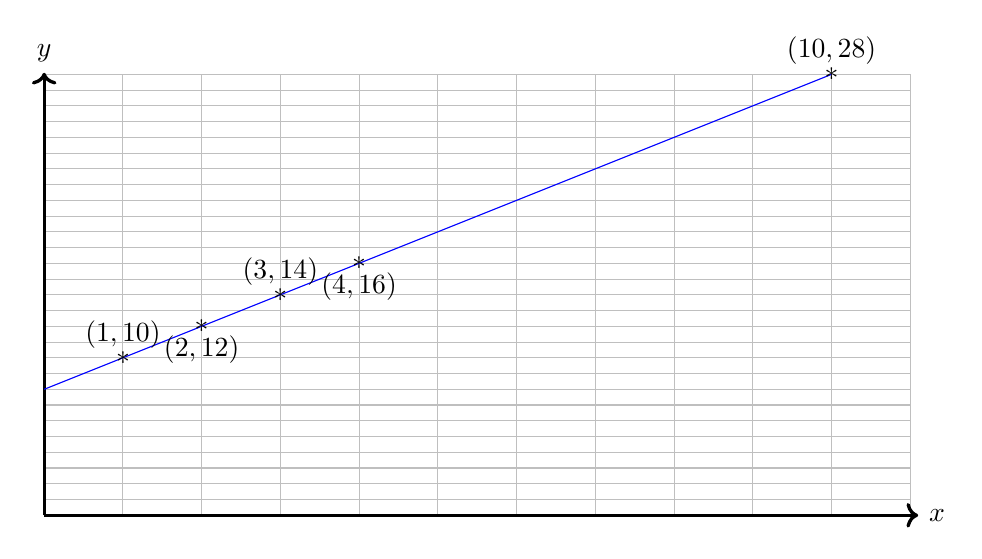
\begin{tikzpicture}[yscale=.2][domain=-0:11]
    \draw[gray!50, thin, step=1] (0,0) grid (11,28);
    \draw[very thick,->] (0,0) -- (11.1,0) node[right] {$x$};
    \draw[very thick,->] (0,0) -- (0,28.1) node[above] {$y$};

%    \foreach \x in {0,...,11} \draw (\x,0.05) -- (\x,-0.05) node[below] {\tiny\x};
%    \foreach \y in {0,...,28} \draw (-0.05,\y) -- (0.05,\y) node[right] {\tiny\y};


  \draw[scale=1,domain=0:10,smooth,variable=\x,blue] plot ({\x},{2*\x+8});

\node at (1,10){$*$};
\draw (1,10) --node[above]{$(1,10)$}(1,10);

\node at (2,12){$*$};
\draw (2,12) --node[below]{$(2,12)$}(2,12);

\node at (3,14){$*$};
\draw (3,14) --node[above]{$(3,14)$}(3,14);

\node at (4,16){$*$};
\draw (4,16) --node[below]{$(4,16)$}(4,16);

\node at (10,28){$*$};
\draw (10,28) --node[above]{$(10,28)$}(10,28);




\end{tikzpicture}$$ % of mbox

An interactive version of this graph may be found here: \url{https://www.desmos.com/calculator/9hocfhhs1m}.


\end{example}


It always helps to illustrate a concept with a \textbf{non}-example.

\begin{example}
Consider a function who takes on the following values:

$$\begin{array}{|c||c|c|c|c|c|}
\hline
x & -2&-1&0&1&2\\
\hline
f(x)&4&1&0&1&4\\
\hline
\end{array}
$$

\textbf{Question:} Does this function appear linear?\\

\textbf{Solution:}If we observe the change from $x=-2$ to $x=-1$, the change in $f(x)$ or $\Delta f(x)=1-4=-3$. 

 However, when we go from $x=-1$ to $x=0$, we see that $\Delta f(x)=0-1=-1$.  Similarly,   when we go from $x=0$ to $x=1$, we see that $\Delta f(x)=1-0=1$, and when we go from $x=1$ to $x=2$, we see that $\Delta f(x)=4-1=3$.
 
 Thus, this function goes from decreasing, to increasing, and the rate at which it does so changes, thus this function is \textbf{not} a linear function.


Graphically we can visualize this:

$$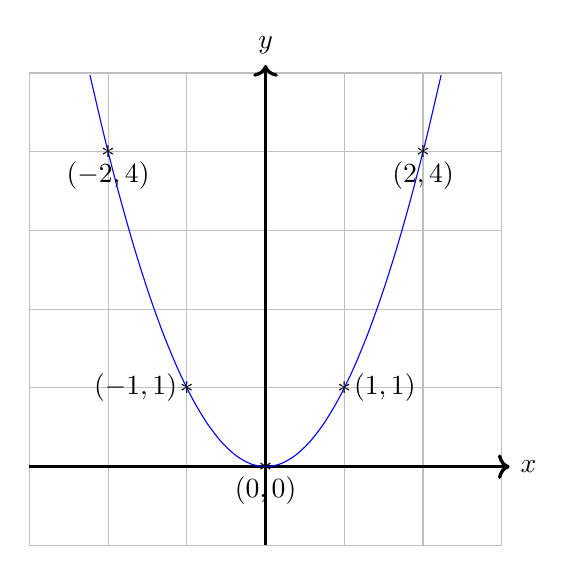
\begin{tikzpicture}[scale=1][domain=-0:11]
    \draw[gray!50, thin, step=1] (-3,-1) grid (3,5);
    \draw[very thick,->] (-3,0) -- (3.1,0) node[right] {$x$};
    \draw[very thick,->] (0,-1) -- (0,5.1) node[above] {$y$};

%    \foreach \x in {0,...,11} \draw (\x,0.05) -- (\x,-0.05) node[below] {\tiny\x};
%    \foreach \y in {0,...,28} \draw (-0.05,\y) -- (0.05,\y) node[right] {\tiny\y};


  \draw[scale=1,domain=-2.23:2.23,smooth,variable=\x,blue] plot ({\x},{\x*\x});

\node at (-2,4){$*$};
\draw (-2,4) --node[below]{$(-2,4)$}(-2,4);

\node at (-1,1){$*$};
\draw (-1,1) --node[left]{$(-1,1)$}(-1,1);

\node at (0,0){$*$};
\draw (0,0) --node[below]{$(0,0)$}(0,0);

\node at (1,1){$*$};
\draw (1,1) --node[right]{$(1,1)$}(1,1);

\node at (2,4){$*$};
\draw (2,4) --node[below]{$(2,4)$}(2,4);




\end{tikzpicture}$$ % of mbox

An interactive version of this graph may be found here: \url{https://www.desmos.com/calculator/za4t3zanlr}.


\end{example}


We can see from the above examples that linear functions are the functions whose graphs may be represented with a straight line.  This is sensible: after all, straight lines move in the same direction, and neither deviate one way nor another, just as linear functions increase, stay constant or decrease at a constant rate.  This is where the name \textbf{linear} functions come from.\\


\section{Standard form and graphs of Linear Functions.}

Algebraically, linear functions are expressible as:

\begin{eqnarray*}
y&=&mx+b, \text{or}\\
f(x)&=&mx+b.
\end{eqnarray*}
%
Where $m$ is the \textbf{slope}, the rate of change of our linear function, and $b$ is the $\mathbf{y}$\textbf{-intercept}.\\



\textbf{Question:} What are these things, why do they have these names, and what do they signify?\\


\subsection{Slope.}


The \textbf{slope} is the constant rate of change of the linear function.  It is often expressed: $$m=\frac{\Delta y}{\Delta x}, m=\frac{\Delta f(x)}{\Delta x}.$$

These algebraic expressions are just a formal way of saying, ``However much $x$ changes, $y$ or $f(x)$ always changes by a proportional amount, and this amount is $m$."


\begin{example}\label{Example:Slope}
Let $y=-x+4$.  This represents a linear function with $m=-1$ and $b=4$.  To verify, if we compared $x=4$ and $x=1$, we have a change in $x$, $\Delta x=4-1=3$.  To find $\Delta y$, we note that when $x=1, y=-(1)+4=3$ and when $x=4, y=-(4)+4=0$.  Thus $\Delta y=0-3=-3$.  So $m=\frac{\Delta f(x)}{\Delta x}=\frac{-3}{3}=-1$.

This shouldn't depend on which choices of $x$ we made.  If we compared $x=3$ and $x=2$, we have a change in $x$, $\Delta x=3-2=1$.  To find $\Delta y$, we note that when $x=3, y=-(3)+4=1$ and when $x=2, y=-(2)+4=2$.  Thus $\Delta y=1-2=-1$.  So $m=\frac{\Delta f(x)}{\Delta x}=\frac{-1}{1}=-1$.

This can be represented visually:

$$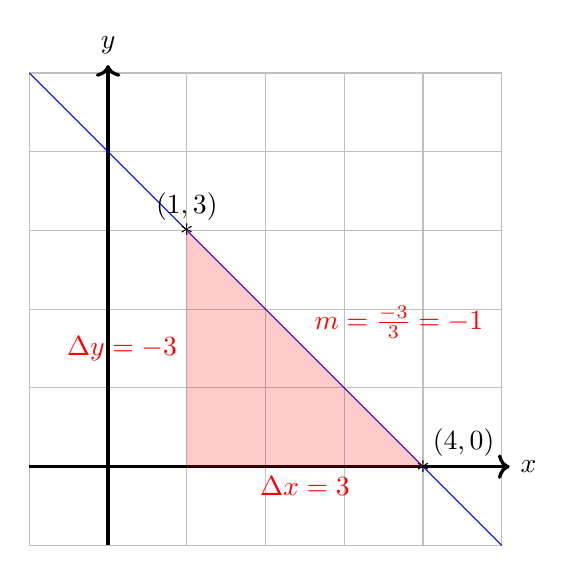
\begin{tikzpicture}[scale=1][domain=-1:5]
    \draw[gray!50, thin, step=1] (-1,-1) grid (5,5);
    \draw[very thick,->] (-1,0) -- (5.1,0) node[right] {$x$};
    \draw[very thick,->] (0,-1) -- (0,5.1) node[above] {$y$};

%    \foreach \x in {0,...,11} \draw (\x,0.05) -- (\x,-0.05) node[below] {\tiny\x};
%    \foreach \y in {0,...,28} \draw (-0.05,\y) -- (0.05,\y) node[right] {\tiny\y};


  \draw[scale=1,domain=-1:5,smooth,variable=\x,blue] plot ({\x},{-1*\x+4});

\node at (1,3){$*$};
\draw (1,3) --node[above]{$(1,3)$}(1,3);

\node at (4,0){$*$};
\draw (4,0) --node[above right]{$(4,0)$}(4,0);

\draw[red, fill, opacity=0.2] (1,3)--(4,0)--(1,0)--(1,3);

\draw[red] (1,1.5) --node[left]{$\Delta y =-3$}(1,1.5);

\draw[red] (2.5,0) --node[below]{$\Delta x =3$}(2.5,0);

\draw[red] (2.5,1.5) --node[above right]{$m=\frac{-3}{3}=-1$}(2.5,1.5);




\end{tikzpicture}%
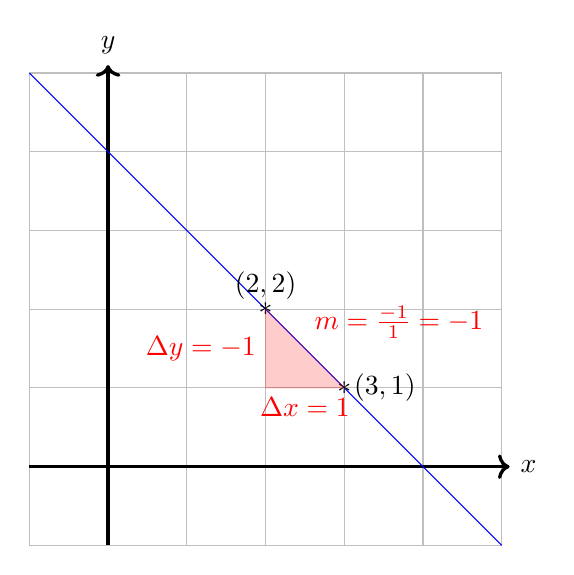
\begin{tikzpicture}[scale=1][domain=-1:5]
    \draw[gray!50, thin, step=1] (-1,-1) grid (5,5);
    \draw[very thick,->] (-1,0) -- (5.1,0) node[right] {$x$};
    \draw[very thick,->] (0,-1) -- (0,5.1) node[above] {$y$};

%    \foreach \x in {0,...,11} \draw (\x,0.05) -- (\x,-0.05) node[below] {\tiny\x};
%    \foreach \y in {0,...,28} \draw (-0.05,\y) -- (0.05,\y) node[right] {\tiny\y};


  \draw[scale=1,domain=-1:5,smooth,variable=\x,blue] plot ({\x},{-1*\x+4});

\node at (2,2){$*$};
\draw (2,2) --node[above]{$(2,2)$}(2,2);

\node at (3,1){$*$};
\draw (3,1) --node[right]{$(3,1)$}(3,1);

\draw[red, fill, opacity=0.2] (2,2)--(3,1)--(2,1)--(2,2);

\draw[red] (2,1.5) --node[left]{$\Delta y =-1$}(2,1.5);

\draw[red] (2.5,1) --node[below]{$\Delta x =1$}(2.5,1);

\draw[red] (2.5,1.5) --node[above right]{$m=\frac{-1}{1}=-1$}(2.5,1.5);




\end{tikzpicture}$$ % of mbox


An interactive version of this graph can be found here:  \url{https://www.desmos.com/calculator/9s3kfotxne}.



\end{example}

\begin{example}\label{Example:NullSlope}
Let $y=3$.  We can re-imagine this as $y=0x+3$, so this represents a linear function with $m=0$ and $b=3$.  Note that no matter what the $x$ values are, $y=3$.  So $\Delta y=0$, and $m=\frac{\Delta y}{\Delta x}=\frac{0}{\Delta x}=0$.  Intuitively, $y$ is always 3 and never changes, so the ``rate of change" is a constant nothing.  This gives us a horizontal line.

This can be represented visually:

$$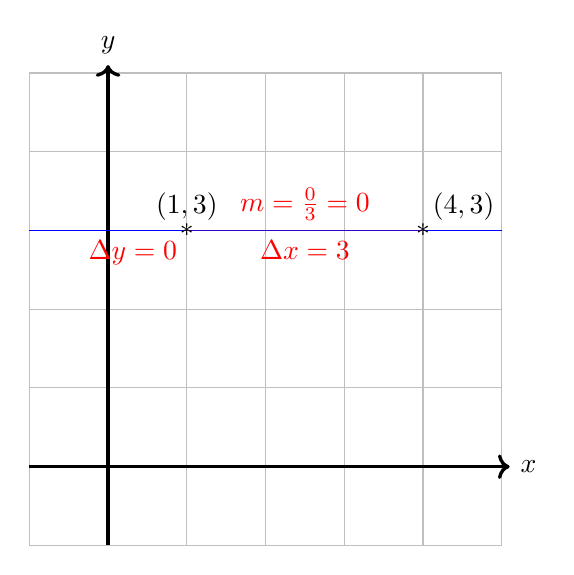
\begin{tikzpicture}[scale=1][domain=-1:5]
    \draw[gray!50, thin, step=1] (-1,-1) grid (5,5);
    \draw[very thick,->] (-1,0) -- (5.1,0) node[right] {$x$};
    \draw[very thick,->] (0,-1) -- (0,5.1) node[above] {$y$};


  \draw[scale=1,domain=-1:5,smooth,variable=\x,blue] plot ({\x},{3});

\node at (1,3){$*$};
\draw (1,3) --node[above]{$(1,3)$}(1,3);

\node at (4,3){$*$};
\draw (4,3) --node[above right]{$(4,3)$}(4,3);

\draw[red, opacity=0.2] (1,3)--(4,3);

\draw[red] (1,3) --node[below left]{$\Delta y =0$}(1,3);

\draw[red] (2.5,3) --node[below]{$\Delta x =3$}(2.5,3);

\draw[red] (2.5,3) --node[above]{$m=\frac{0}{3}=0$}(2.5,3);



\end{tikzpicture}%
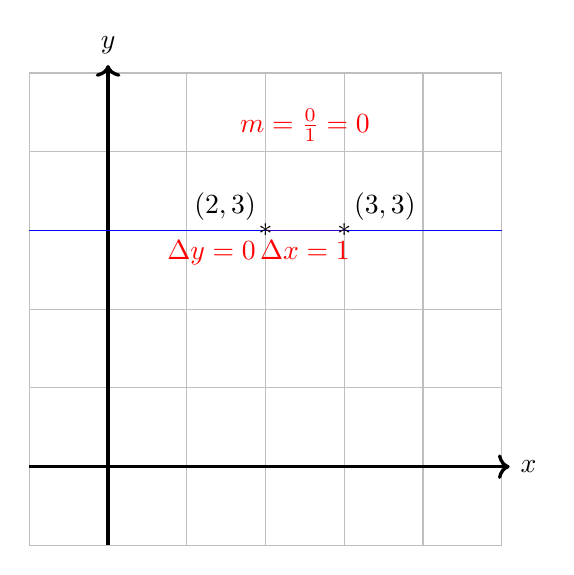
\begin{tikzpicture}[scale=1][domain=-1:5]
    \draw[gray!50, thin, step=1] (-1,-1) grid (5,5);
    \draw[very thick,->] (-1,0) -- (5.1,0) node[right] {$x$};
    \draw[very thick,->] (0,-1) -- (0,5.1) node[above] {$y$};


  \draw[scale=1,domain=-1:5,smooth,variable=\x,blue] plot ({\x},{3});

\node at (2,3){$*$};
\draw (2,3) --node[above left]{$(2,3)$}(2,3);

\node at (3,3){$*$};
\draw (3,3) --node[above right]{$(3,3)$}(3,3);

\draw[red, opacity=0.2] (2,3)--(3,3);

\draw[red] (2,3) --node[below left]{$\Delta y =0$}(2,3);

\draw[red] (2.5,3) --node[below]{$\Delta x =1$}(2.5,3);

\draw[red] (2.5,4) --node[above]{$m=\frac{0}{1}=0$}(2.5,4);




\end{tikzpicture}%
$$ % of mbox


An interactive version of this graph can be found here:  \url{https://www.desmos.com/calculator/pv7m6fbugb}.



\end{example}

\subsection{$\mathbf{y}$-intercept.}

The $\mathbf{y}$\textbf{-intercept} of a linear function $y=mx+b$ is the value $b$.  It is so named because it is the value of the linear function when it \textbf{intercepts} the $y$-axis.  The reason for this is that the $y$-axis is exactly the line $x=0$, and when $x=0$, $y=m(0)+b=b$.


\begin{example}\label{Example:Intercept}
Let us recall Example \ref{Example:Slope} and let $y=-x+4$.  Note that when $x=0, y=-(0)+4=4$.

This can be represented visually:

$$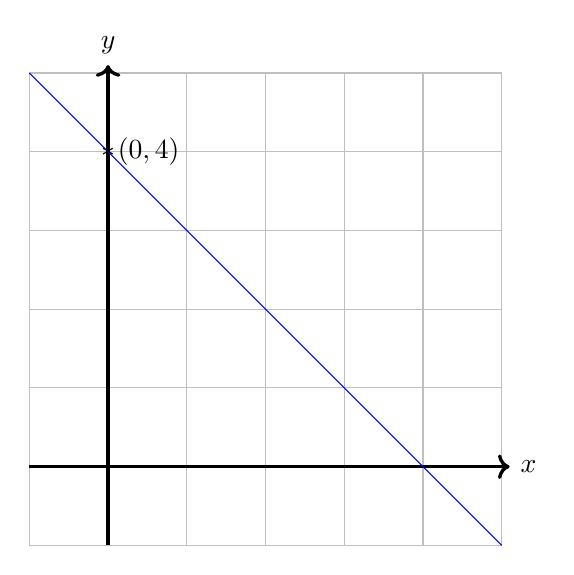
\begin{tikzpicture}[scale=1][domain=-1:5]
    \draw[gray!50, thin, step=1] (-1,-1) grid (5,5);
    \draw[very thick,->] (-1,0) -- (5.1,0) node[right] {$x$};
    \draw[very thick,->] (0,-1) -- (0,5.1) node[above] {$y$};

%    \foreach \x in {0,...,11} \draw (\x,0.05) -- (\x,-0.05) node[below] {\tiny\x};
%    \foreach \y in {0,...,28} \draw (-0.05,\y) -- (0.05,\y) node[right] {\tiny\y};


  \draw[scale=1,domain=-1:5,smooth,variable=\x,blue] plot ({\x},{-1*\x+4});

\node at (0,4){$*$};
\draw (0,4) --node[right]{$(0,4)$}(0,4);





\end{tikzpicture}$$ % of mbox


Note that $4$ is the height of the function when it intercepts the $y$-axis.


\end{example}

\begin{example}\label{Example:Intercept}
Let us recall Example \ref{Example:NullSlope} and let $y=3=0x+3$.  Note that when $x=0, y=3$.

This can be represented visually:

$$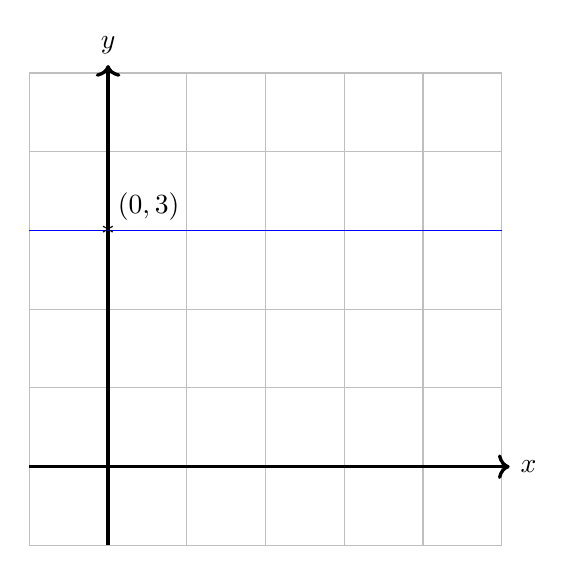
\begin{tikzpicture}[scale=1][domain=-1:5]
    \draw[gray!50, thin, step=1] (-1,-1) grid (5,5);
    \draw[very thick,->] (-1,0) -- (5.1,0) node[right] {$x$};
    \draw[very thick,->] (0,-1) -- (0,5.1) node[above] {$y$};

%    \foreach \x in {0,...,11} \draw (\x,0.05) -- (\x,-0.05) node[below] {\tiny\x};
%    \foreach \y in {0,...,28} \draw (-0.05,\y) -- (0.05,\y) node[right] {\tiny\y};


  \draw[scale=1,domain=-1:5,smooth,variable=\x,blue] plot ({\x},{3});

\node at (0,3){$*$};
\draw (0,3) --node[above right]{$(0,3)$}(0,3);





\end{tikzpicture}$$ % of mbox


Note that $3$ is the height of the function when it intercepts the $y$-axis.


\end{example}


\subsection{Translating from Algebra to Geometry}

We can see in our above examples that linear functions have both an algebraic form and a geometric interpretation.   Both are useful and in fact necessary to understand what's going on with a linear function.  So what we now want to ask ourselves is, given the algebraic expression for a line, how might we find it's geometric representation?\\


Intuitively, we know that if we had a sheet of paper and a ruler, if we drew 2 points on this paper, we could find the line between them.  So to find a geometric representation of a linear function, we should:

\begin{enumerate}
    \item Find a point that must be on thee line.
    \item Identify a second point on the line.
    \item Draw the line between them.
\end{enumerate}

\begin{example}\label{Example:DrawLine}
\textbf{Question:} Draw the line $y=f(x)$ where $f(x)=-\frac{2}{3}x+4$.

\begin{enumerate}
    \item We first identify a point on the line, the easiest to find is probably the $y$-intercept, note that when $x=0, f(x)=-\frac{2}{3}(0)+4=4$, thus $(0,4)$ is on $y=f(x)$.
    \item We have infinitely many choices for a second point, but to make the arithmetic easy, let's let $x=3$, then $f(x)=-\frac{2}{3}(3)+4=-2+4=2$, so $(3,2)$ is on the line.
    
    Note this gives us:
 $$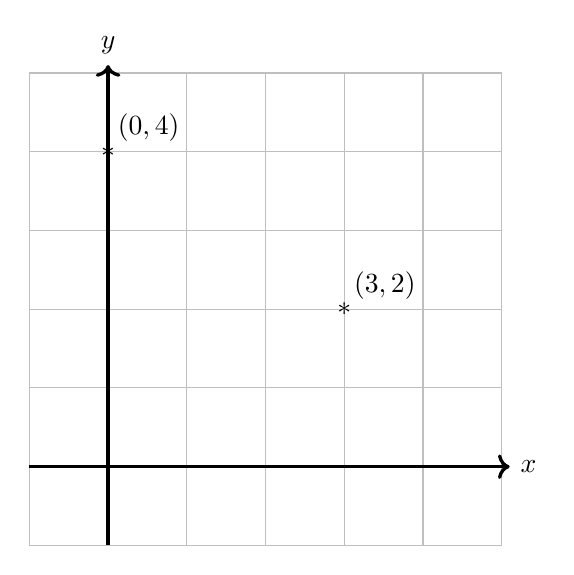
\begin{tikzpicture}[scale=1][domain=-1:5]
    \draw[gray!50, thin, step=1] (-1,-1) grid (5,5);
    \draw[very thick,->] (-1,0) -- (5.1,0) node[right] {$x$};
    \draw[very thick,->] (0,-1) -- (0,5.1) node[above] {$y$};

%    \foreach \x in {0,...,11} \draw (\x,0.05) -- (\x,-0.05) node[below] {\tiny\x};
%    \foreach \y in {0,...,28} \draw (-0.05,\y) -- (0.05,\y) node[right] {\tiny\y};


%  \draw[scale=1,domain=-1:5,smooth,variable=\x,blue] plot ({\x},{(-2/3)*\x+4});

\node at (0,4){$*$};
\draw (0,4) --node[above right]{$(0,4)$}(0,4);

\node at (3,2){$*$};
\draw (3,2) --node[above right]{$(3,2)$}(3,2);




\end{tikzpicture}$$    
    \item We then literally connect the dots:
$$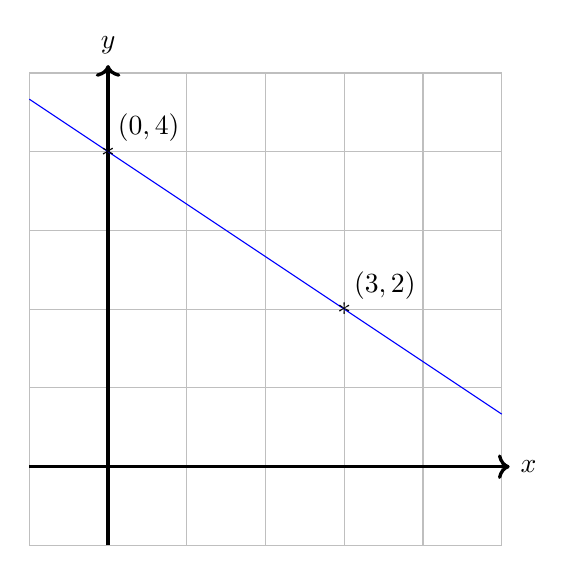
\begin{tikzpicture}[scale=1][domain=-1:5]
    \draw[gray!50, thin, step=1] (-1,-1) grid (5,5);
    \draw[very thick,->] (-1,0) -- (5.1,0) node[right] {$x$};
    \draw[very thick,->] (0,-1) -- (0,5.1) node[above] {$y$};

%    \foreach \x in {0,...,11} \draw (\x,0.05) -- (\x,-0.05) node[below] {\tiny\x};
%    \foreach \y in {0,...,28} \draw (-0.05,\y) -- (0.05,\y) node[right] {\tiny\y};


  \draw[scale=1,domain=-1:5,smooth,variable=\x,blue] plot ({\x},{(-2/3)*\x+4});

\node at (0,4){$*$};
\draw (0,4) --node[above right]{$(0,4)$}(0,4);

\node at (3,2){$*$};
\draw (3,2) --node[above right]{$(3,2)$}(3,2);




\end{tikzpicture}$$      
\end{enumerate}
Modern technology also let's us readily draw these functions: \url{https://www.desmos.com/calculator/gyvulordwz}.
\end{example}

\begin{example}\label{Example:DrawLineOtherForm}
\textbf{Question:} Draw the line $2x+4y=8$.

\begin{enumerate}
    \item We first identify a point on the line.  To make life easy note that when $x=0, 2(0)+4y=8$ and $y=2$, thus $(0,2)$ is on $2x+4y=8$.
    \item Similarly when $y=0, 2x+4(0)=8$ and $x=4$, thus $(4,0)$ is on $2x+4y=8$.
    
    Note this gives us:
 $$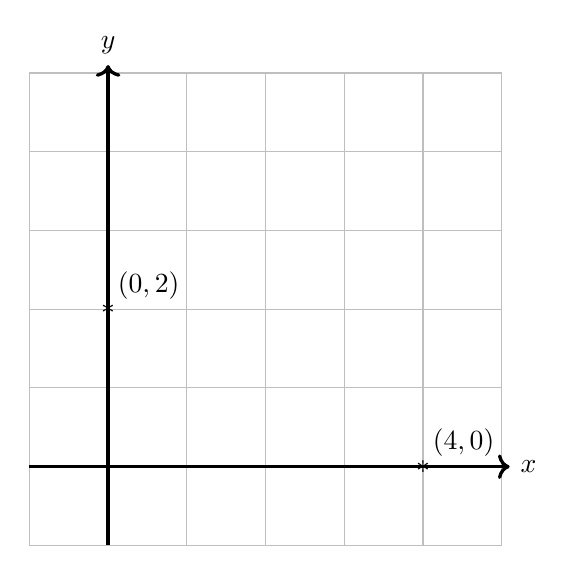
\begin{tikzpicture}[scale=1][domain=-1:5]
    \draw[gray!50, thin, step=1] (-1,-1) grid (5,5);
    \draw[very thick,->] (-1,0) -- (5.1,0) node[right] {$x$};
    \draw[very thick,->] (0,-1) -- (0,5.1) node[above] {$y$};

%    \foreach \x in {0,...,11} \draw (\x,0.05) -- (\x,-0.05) node[below] {\tiny\x};
%    \foreach \y in {0,...,28} \draw (-0.05,\y) -- (0.05,\y) node[right] {\tiny\y};


%  \draw[scale=1,domain=-1:5,smooth,variable=\x,blue] plot ({\x},{(-1/2)*\x+2});

\node at (0,2){$*$};
\draw (0,2) --node[above right]{$(0,2)$}(0,2);

\node at (4,0){$*$};
\draw (4,0) --node[above right]{$(4,0)$}(4,0);




\end{tikzpicture}$$    
    \item We then connect the dots:
$$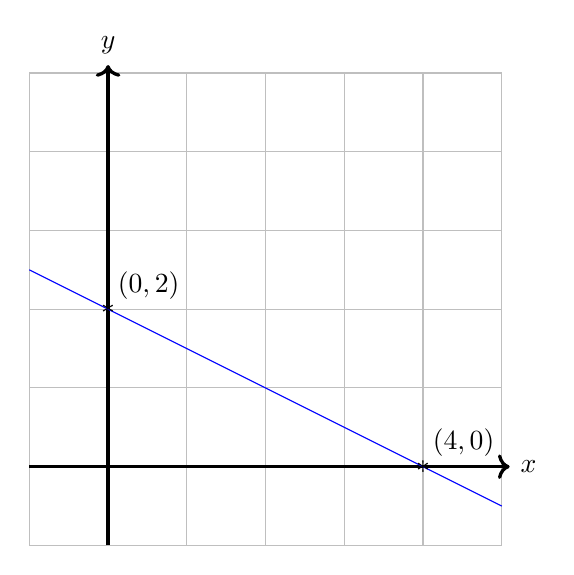
\begin{tikzpicture}[scale=1][domain=-1:5]
    \draw[gray!50, thin, step=1] (-1,-1) grid (5,5);
    \draw[very thick,->] (-1,0) -- (5.1,0) node[right] {$x$};
    \draw[very thick,->] (0,-1) -- (0,5.1) node[above] {$y$};

%    \foreach \x in {0,...,11} \draw (\x,0.05) -- (\x,-0.05) node[below] {\tiny\x};
%    \foreach \y in {0,...,28} \draw (-0.05,\y) -- (0.05,\y) node[right] {\tiny\y};


  \draw[scale=1,domain=-1:5,smooth,variable=\x,blue] plot ({\x},{(-1/2)*\x+2});

\node at (0,2){$*$};
\draw (0,2) --node[above right]{$(0,2)$}(0,2);

\node at (4,0){$*$};
\draw (4,0) --node[above right]{$(4,0)$}(4,0);




\end{tikzpicture}$$          
\end{enumerate}
Again, utilizing technology: \url{https://www.desmos.com/calculator/lprlevpf6q}.\\

Note that we could have taken $2x+4y=8$ and rewritten it:

\begin{eqnarray*}
2x+4y&=&8\\
4y&=&-2x+8\\
y&=&-\frac{1}{2}x+2,
\end{eqnarray*}

and from here, treated it the same way as in Example \ref{Example:DrawLine}.

\end{example}



\section{Identifying a Linear Function from information.}


It is often the case that when one works with a linear function, one will not be given the exact form for the function.  You may for example only know the rate of change, or the value of the function at a few points.  To be able to make the most of this situation, it would be good to be able to still identify the linear function in question, when possible.\\

\textbf{Question:}  What is the minimal amount of information necessary to identify a linear function?\\

Here is where our geometric interpretation of these functions is helpful.  If someone handed you a sheet of paper and asked you to draw a line, how much information would they have to give you so there could be only one like you'd be able to draw?\\

\textbf{Question:}  Is a point enough?\\

If someone drew a dot on a piece of paper, there is certainly a line you could draw through it, but it definitely does seem like there's infinitely many lines you could draw as well.  Take $(2,3)$:

$$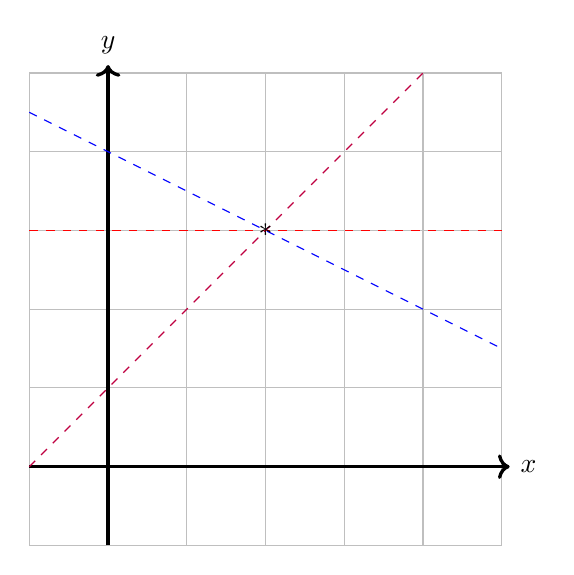
\begin{tikzpicture}[scale=1][domain=-1:5]
    \draw[gray!50, thin, step=1] (-1,-1) grid (5,5);
    \draw[very thick,->] (-1,0) -- (5.1,0) node[right] {$x$};
    \draw[very thick,->] (0,-1) -- (0,5.1) node[above] {$y$};

%    \foreach \x in {0,...,11} \draw (\x,0.05) -- (\x,-0.05) node[below] {\tiny\x};
%    \foreach \y in {0,...,28} \draw (-0.05,\y) -- (0.05,\y) node[right] {\tiny\y};


    \draw[scale=1,domain=-1:5,smooth,variable=\x,blue, dashed] plot ({\x},{(-1/2)*\x+4});
  
    \draw[scale=1,domain=-1:5,smooth,variable=\x,red, dashed] plot ({\x},{3});
    
    \draw[scale=1,domain=-1:4,smooth,variable=\x,purple, dashed] plot ({\x},{\x+1});

\node at (2,3){$*$};

\end{tikzpicture}$$   

Of course there are many more, here's a visualization: \url{https://www.desmos.com/calculator/c3gronrfd3}.



\textbf{Question:}  Is a slope/direction enough?\\

If someone gave you a piece of paper and told you would direction the line should take, there is definitely a line you could draw with that direction, but depending where you start, there's infinitely many lines you could draw as well.  Take $m=\frac{3}{2}$:

$$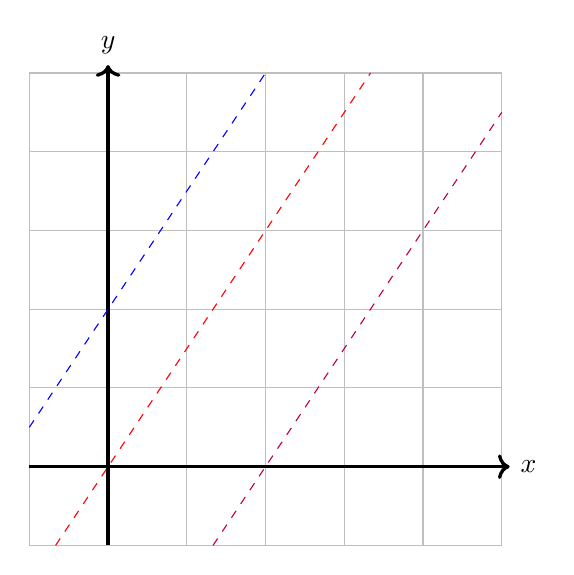
\begin{tikzpicture}[scale=1][domain=-1:5]
    \draw[gray!50, thin, step=1] (-1,-1) grid (5,5);
    \draw[very thick,->] (-1,0) -- (5.1,0) node[right] {$x$};
    \draw[very thick,->] (0,-1) -- (0,5.1) node[above] {$y$};

%    \foreach \x in {0,...,11} \draw (\x,0.05) -- (\x,-0.05) node[below] {\tiny\x};
%    \foreach \y in {0,...,28} \draw (-0.05,\y) -- (0.05,\y) node[right] {\tiny\y};


    \draw[scale=1,domain=-1:2,smooth,variable=\x,blue, dashed] plot ({\x},{(3/2)*\x+2});
  
    \draw[scale=1,domain=-2/3:10/3,smooth,variable=\x,red, dashed] plot ({\x},{(3/2)*\x});
    
    \draw[scale=1,domain=4/3:5,smooth,variable=\x,purple, dashed] plot ({\x},{(3/2)*\x-3});


\end{tikzpicture}$$   

Of course there are many more, here's a visualization: \url{https://www.desmos.com/calculator/iwcjwhen1b}.


So this begs the question, what \textbf{IS} the mininum amount of information that you'd need to uniquely identify a line?

\subsection{Point \& Slope}

If we combined the two pieces of information from the start of the section, would we obtain a unique line?  Intuitively this should make sense, there are infinitely many lines which go through a point, but only one with slope $m=\frac{3}{2}$, similarly, there are infinitely many lines with slope $\frac{3}{2}$, but they all pass through different points, only one of them passes through $(2,3)$.  Again to refer to our geometric ideas, if someone drew a point on a paper, and told you which direction you had to go from there, there's really only one line you could draw.\\

Here are some visualizations:  

$$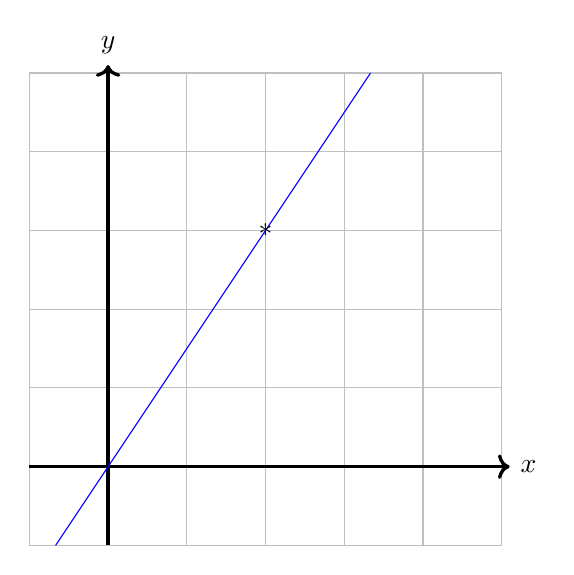
\begin{tikzpicture}[scale=1][domain=-1:5]
    \draw[gray!50, thin, step=1] (-1,-1) grid (5,5);
    \draw[very thick,->] (-1,0) -- (5.1,0) node[right] {$x$};
    \draw[very thick,->] (0,-1) -- (0,5.1) node[above] {$y$};



%    \foreach \x in {0,...,11} \draw (\x,0.05) -- (\x,-0.05) node[below] {\tiny\x};
%    \foreach \y in {0,...,28} \draw (-0.05,\y) -- (0.05,\y) node[right] {\tiny\y};


    \draw[scale=1,domain=-2/3:10/3,smooth,variable=\x,blue] plot ({\x},{(3/2)*\x});
  

\node at (2,3){$*$};

\end{tikzpicture}$$   



\url{https://www.desmos.com/calculator/5ikul0ktn5}, \url{https://www.desmos.com/calculator/hcl8ynd0yp}.

\textbf{Question:} How does this translate Algebraically?

So given a linear function is defined by the slope $m$ and intercept $b$.  By the discussion above, if we are given a slope $\textcolor{red}{m}$ and a pair of points $\textcolor{blue}{(x_0,y_0)}$, we should be able to uniquely identify $b$.

\begin{example}\label{Example:PandS}
\textbf{Question:}  Find the linear function with slope 3 passing through $(2,5)$.\\

Note that we are given $\textcolor{red}{m=3}$ and $\textcolor{blue}{(x_0,y_0)=(2,5)}$.  The general form for a line is $y=mx+b$, thus:

\begin{eqnarray*}
y&=&mx+b\\
\textcolor{blue}{5}&=&\textcolor{red}{3}\cdot\textcolor{blue}{2}+b\\
5&=&6+b\\
b&=&5-6=-1.\\
\end{eqnarray*}

Thus $y=3x-1$ is the linear equation in question, $m=3, b=-1$.

$$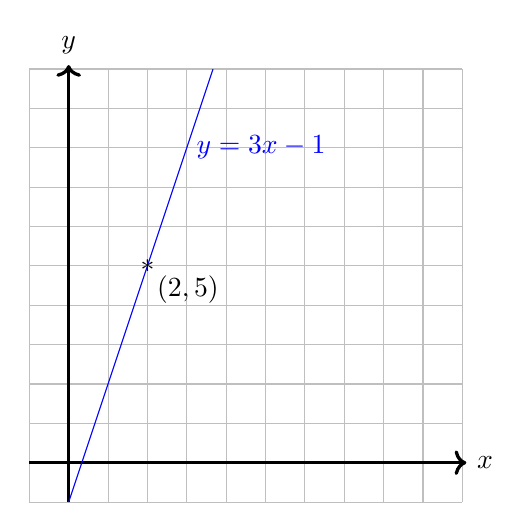
\begin{tikzpicture}[scale=0.5][domain=-1:10]
    \draw[gray!50, thin, step=1] (-1,-1) grid (10,10);
    \draw[very thick,->] (-1,0) -- (10.1,0) node[right] {$x$};
    \draw[very thick,->] (0,-1) -- (0,10.1) node[above] {$y$};

%    \foreach \x in {0,...,11} \draw (\x,0.05) -- (\x,-0.05) node[below] {\tiny\x};
%    \foreach \y in {0,...,28} \draw (-0.05,\y) -- (0.05,\y) node[right] {\tiny\y};


    \draw[scale=1,domain=0:3.666,smooth,variable=\x,blue] plot ({\x},{(3)*\x-1});
  

\node at (2,5){$*$};
\draw (2,5) --node[below right]{$(2,5)$}(2,5);
\draw[blue] (3,8) --node[right]{$y=3x-1$}(3,8);



\end{tikzpicture}$$   
\url{https://www.desmos.com/calculator/w3nixbtfrs}.

We can verify that this line has slope $m=3$ and when $x=2, y=3\cdot 2-1=6-1=5$.

\end{example}


\subsection{Point-Slope form.}

So, typically lines are defined in the form $y=mx+b$, where $m$ is the slope and $b$ is the $y$-intercept.  It can be convenient to also define a line in the form $$y-y_0=m(x-x_0),$$ where $(x_0, y_0)$ is a point that falls on your line.\\

Why would we care about a second formulation, and how do we know it's even a line?  To answer the first question, we recall that ANY geometric object defined by an equation is the set of points that make the equation true.  So given the equation $y-y_0=m(x-x_0)$, if we plug in $(x_0, y_0)$, we would get $y_0-y_0=m(x_0-x_0)$ or $0=0$ which is definitely a true statement.  So whatever shape we get from $y-y_0=m(x-x_0)$, it contains $(x_0, y_0)$.\\

We know it's a line because:

\begin{eqnarray*}
y-y_0&=&m(x-x_0)\\
y&=&mx-mx_0+y_0\\
y&=&mx+(y_0-mx_0)
\end{eqnarray*}

so if we let $b=y_0-mx_0$, we get the standard form for a line.


\begin{example}\label{Example:PandSagain}
\textbf{Question:} Find the line with slope 3 passing through $(2,5)$, again.\\

Using the point-slope form, knowing that $\textcolor{blue}{(2,5)}$ lies on the line, and that $\textcolor{red}{m}$:

\begin{eqnarray*}
y-y_0&=&m(x-x_0)\\
y-\textcolor{blue}{5}&=&\textcolor{red}{3}(x-\textcolor{blue}{2})\\
y&=&3x-6+5\\
y&=&3x-1.
\end{eqnarray*}

Either way, you obtain the same line, with slope 3, passing through (2,5).

\end{example}

\subsection{Two Points}

On the other hand, instead of giving you a point and a direction, one could be given two points to traverse through.  If you imagine any two dots on a piece of paper, one can imagine that you may draw a line between them.  The exact way we do this also follows intuitively.  If you were at home, and you had to go to the store, the natural steps you would take to do so are:

\begin{enumerate}
\item Figure out which way to the store.
\item Go there.
\end{enumerate}

So we have to figure out the direction between these points, which in our analogy means the slope between the points.  Remember the slope measures how much $y$ changes per change in $x$, or $m=\frac{\Delta y}{\Delta x}$.  So, the measurement of slope follows from the change in $y$ over the change in $x$.  So to measure this, if we have points $(x_0, y_0), (x_1, y_1)$, we want to see how much $y$ changes over how much $x$ changes, or:

$$m=\frac{\Delta y}{\Delta x}=\frac{y_1-y_0}{x_1-x_0}$$
or equivalently $m=\frac{y_0-y_1}{x_0-x_1}$.


\begin{example}\label{Example:PandP}
What line passes between $(2,3)$ and $(4,1)$?\\

So we note then that $\textcolor{red}{m=\frac{1-3}{4-2}=-1}$ (also $\textcolor{red}{m=\frac{3-1}{2-4}=-1}$).  Once the slope is identified, we can use any point, and any method to find the line.  Once we pick a point, We have a problem that follows the form of Examples \ref{Example:PandS}, \ref{Example:PandSagain}.

We won't go through all the possibilities but if we considered the point $\textcolor{blue}{(2,3)}$:

\begin{eqnarray*}
y&=&mx+b\\
\textcolor{blue}{3}&=&\textcolor{red}{-1}\cdot \textcolor{blue}{2}+b\\
b&=&3+2=5\\
y&=&-x+5.
\end{eqnarray*}

Or if we picked $\textcolor{blue}{(1,4)}$:

\begin{eqnarray*}
y-y_0&=&m(x-x_0)\\
y-\textcolor{blue}{1}&=&\textcolor{red}{-1}\cdot(x-\textcolor{blue}{4})\\
y&=&-x+4+1\\
y&=&-x+5.
\end{eqnarray*}

Either way, we identify the same line:

$$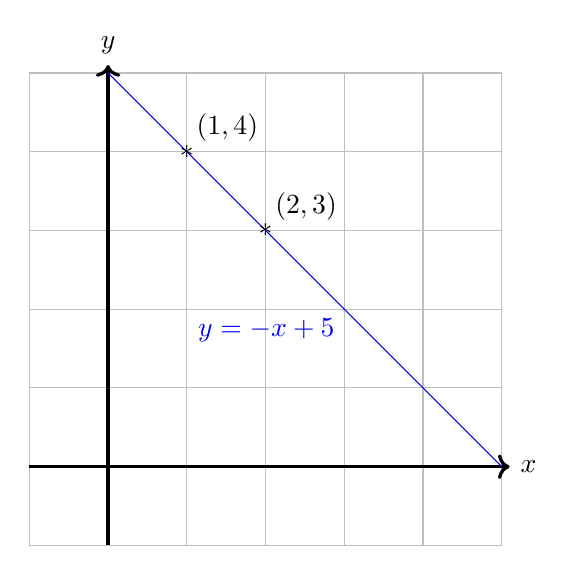
\begin{tikzpicture}[scale=1][domain=-1:5]
    \draw[gray!50, thin, step=1] (-1,-1) grid (5,5);
    \draw[very thick,->] (-1,0) -- (5.1,0) node[right] {$x$};
    \draw[very thick,->] (0,-1) -- (0,5.1) node[above] {$y$};

%    \foreach \x in {0,...,11} \draw (\x,0.05) -- (\x,-0.05) node[below] {\tiny\x};
%    \foreach \y in {0,...,28} \draw (-0.05,\y) -- (0.05,\y) node[right] {\tiny\y};


    \draw[scale=1,domain=0:5,smooth,variable=\x,blue] plot ({\x},{(-1)*\x+5});
  

\node at (2,3){$*$};
\draw (2,3) --node[above right]{$(2,3)$}(2,3);

\node at (1,4){$*$};
\draw (1,4) --node[above right]{$(1,4)$}(1,4);

\draw[blue] (3,2) --node[below left]{$y=-x+5$}(3,2);


\end{tikzpicture}$$  

\url{https://www.desmos.com/calculator/yohrdbuwuc}

\end{example}

\section{Utilizing the Linear Function}

Once you obtain a linear function, this gives you a relationship between the $x$ and $y$ variables.  It allows you to identify, given an $x$ or $y$ value, the other value:

\begin{example}\label{Example:LinearFindValue}
Consider the linear function $y=2x-3$.
\begin{enumerate}
\item When $y=0$, what is $x$?
\item When $x=3$ what is $y$?
\end{enumerate}

These can be identified algebraically:
\begin{enumerate}
\item When $\textcolor{ForestGreen}{y=0}$, we have:
\begin{eqnarray*}
y&=&2x-3\\
\textcolor{ForestGreen}{0}&=&2x-3\\
3&=&2x\\
x&=&1.5.
\end{eqnarray*}
\item If $\textcolor{orange}{x=3}$:
\begin{eqnarray*}
y&=&2x-3\\
y&=&2(\textcolor{orange}{3})-3\\
y&=&6-3=3.
\end{eqnarray*}
We can identify both points graphically as well:



\url{https://www.desmos.com/calculator/gukgr4sjfm}.
\end{enumerate}

$$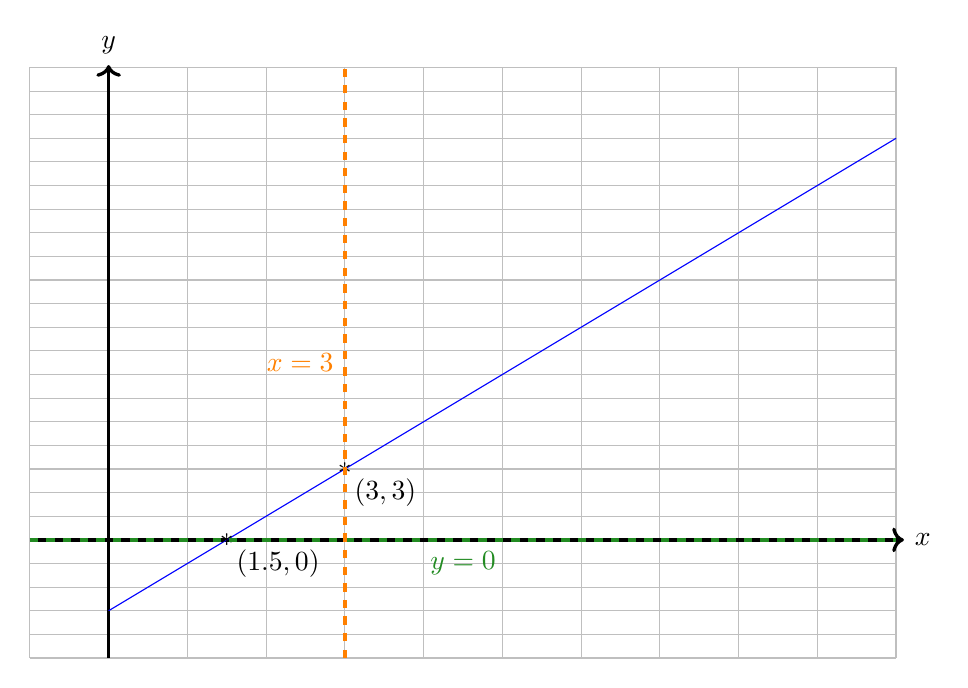
\begin{tikzpicture}[yscale=0.3][domain=-1:10]
    \draw[gray!50, thin, step=1] (-1,-5) grid (10,20);
    \draw[very thick,->] (-1,0) -- (10.1,0) node[right] {$x$};
    \draw[very thick,->] (0,-5) -- (0,20.1) node[above] {$y$};

%    \foreach \x in {0,...,11} \draw (\x,0.05) -- (\x,-0.05) node[below] {\tiny\x};
%    \foreach \y in {0,...,28} \draw (-0.05,\y) -- (0.05,\y) node[right] {\tiny\y};


    \draw[scale=1,domain=0:10,smooth,variable=\x,blue] plot ({\x},{(2)*\x-3});
  

\node at (1.5,0){$*$};
\draw (1.5,0) --node[below right]{$(1.5,0)$}(1.5,0);

\node at (3,3){$*$};
\draw (3,3) --node[below right]{$(3,3)$}(3,3);

\draw[ForestGreen, dashed, ultra thick] (-1,0) --node[below]{$y=0$}(10,0);

\draw[orange, dashed, ultra thick] (3,-5) --node[left]{$x=3$}(3,20);


\end{tikzpicture}$$  

\end{example}


\section{Applications of Linear Functions}

Up until this point, we've been treating linear functions as somewhat disembodied Mathematical entities.  In this section, we'll give a few examples to show how they appear and are applied in practice.


\begin{example}\label{Example:LinearTemp}

\Q The freezing point of water is $0^\circ$ Celsius and $32^\circ$ Fahrenheit.  The boiling point of water is $100^\circ$ Celsius and $212^\circ$ Fahrenheit.

\begin{enumerate}
    \item Find a linear function $T(F)=C$ that converts Fahrenheit into Celsius.
    \item When it's 10 degrees Fahrenheit, what is the temperature in Celsius?
    \item When it's 30 degrees Celsius, what is the temperature in Fahrenheit?
\end{enumerate}

\Sol We are given that $T(32)=0$ and $T(212)=100$.  This gives us points $(32,0)$ and $(212,100)$, so this bears some similarity to Example \ref{Example:PandP}.

\begin{enumerate}
    \item We first identify the slope of the function: $$m=\frac{\Delta C}{\Delta F}=\frac{100-0}{212-32}=\frac{100}{180}=\TCR{\frac{5}{9}}.$$
Then choosing either point, say $\TCB{(32,0)}$, and point slope form, we have:
\begin{eqnarray*}
C-C_0&=&m(F-F_0)\\
C-\TCB{0}&=&\TCR{\frac{5}{9}}(F-\TCB{32})\\
C&=&\frac{5}{9}F-\frac{160}{9}.
\end{eqnarray*}

Thus $T(F)=\frac{5}{9}F-\frac{160}{9}$

$$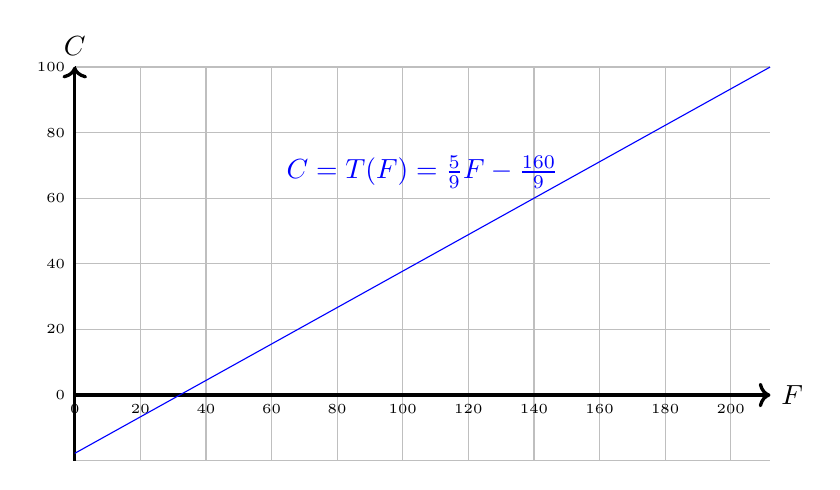
\begin{tikzpicture}[yscale=1/24, xscale=1/24][domain=-1:10]
    \draw[gray!50, thin, step=20] (0,-20) grid (212,100);
    \draw[very thick,->] (0,0) -- (212.1,0) node[right] {$F$};
    \draw[very thick,->] (0,-20) -- (0,100.1) node[above] {$C$};

    \foreach \x in {0,20,...,200} \draw (\x,0.05) -- (\x,-0.05) node[below] {\tiny\x};
    \foreach \y in {0,20,...,100} \draw (-0.05,\y) -- (0.05,\y) node[left] {\tiny\y};


    \draw[scale=1,domain=0:212,smooth,variable=\x,blue] plot ({\x},{(5/9)*\x-160/9});
  

\draw[blue] (106,60) --node[above]{$C=T(F)=\frac{5}{9}F-\frac{160}{9}$}(106,60);


\end{tikzpicture}$$ 

\item When it's 10 degrees, we have that $\TCG{F=10}$ and so:

\begin{eqnarray*}
C&=&\frac{5}{9}F-\frac{160}{9}\\
C&=&\frac{5}{9}\cdot\TCG{10}-\frac{160}{9}\\
C&=&\frac{50}{9}-\frac{160}{9}\\
C&=&-\frac{110}{9}\approx-12.2222.
\end{eqnarray*}
So 10 degrees Fahrenheit is $-\frac{110}{9}\approx-12.2222$ degrees Celsius.

$$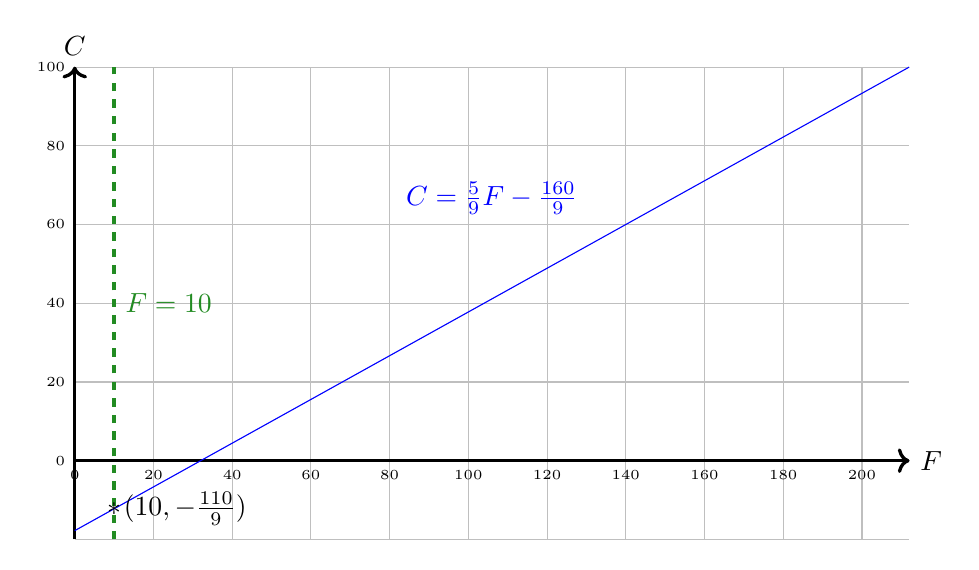
\begin{tikzpicture}[yscale=1/20, xscale=1/20][domain=-1:10]
    \draw[gray!50, thin, step=20] (0,-20) grid (212,100);
    \draw[very thick,->] (0,0) -- (212.1,0) node[right] {$F$};
    \draw[very thick,->] (0,-20) -- (0,100.1) node[above] {$C$};

    \foreach \x in {0,20,...,200} \draw (\x,0.05) -- (\x,-0.05) node[below] {\tiny\x};
    \foreach \y in {0,20,...,100} \draw (-0.05,\y) -- (0.05,\y) node[left] {\tiny\y};


    \draw[scale=1,domain=0:212,smooth,variable=\x,blue] plot ({\x},{(5/9)*\x-160/9});
  

\draw[blue] (106,60) --node[above]{$C=\frac{5}{9}F-\frac{160}{9}$}(106,60);
\draw[ultra thick, dashed, ForestGreen] (10,-20) --node[right]{$F=10$} (10,100);

\node at (10,-12.22222){$*$};
\draw (10,-12.22222) --node[right]{$(10,-\frac{110}{9})$}(10,-12.22222);



\end{tikzpicture}$$ 

\item When it's 30 degrees Celsius i.e.\ $\TCO{C=30}$ we have:

\begin{eqnarray*}
C&=&\frac{5}{9}F-\frac{160}{9}\\
\TCO{30}&=&\frac{5}{9}F-\frac{160}{9}\\
30+\frac{160}{9}&=&\frac{5}{9}F\\
\frac{430}{9}&=&\frac{5}{9}F\\
F&=&\frac{430}{5}=86.
\end{eqnarray*}

So when it's 30 degrees Celsius, it is 86 degrees Fahrenheit.

$$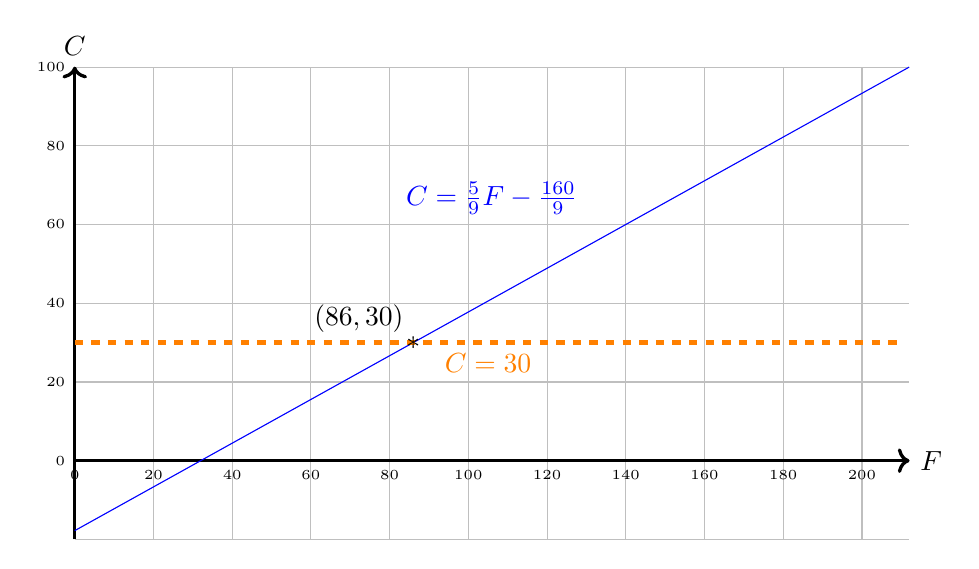
\begin{tikzpicture}[yscale=1/20, xscale=1/20][domain=-1:10]
    \draw[gray!50, thin, step=20] (0,-20) grid (212,100);
    \draw[very thick,->] (0,0) -- (212.1,0) node[right] {$F$};
    \draw[very thick,->] (0,-20) -- (0,100.1) node[above] {$C$};

    \foreach \x in {0,20,...,200} \draw (\x,0.05) -- (\x,-0.05) node[below] {\tiny\x};
    \foreach \y in {0,20,...,100} \draw (-0.05,\y) -- (0.05,\y) node[left] {\tiny\y};


    \draw[scale=1,domain=0:212,smooth,variable=\x,blue] plot ({\x},{(5/9)*\x-160/9});
  

\draw[blue] (106,60) --node[above]{$C=\frac{5}{9}F-\frac{160}{9}$}(106,60);
\draw[ultra thick, dashed, orange] (0,30) --node[below]{$C=30$} (210,30);

\node at (86,30){$*$};
\draw (86,30) --node[above left]{$(86,30)$}(86,30);



\end{tikzpicture}$$ 


\end{enumerate}

Desmos representation here: \url{https://www.desmos.com/calculator/tyoznzrk53}.


\end{example}

\begin{example}\label{Example:Proft}
\Q Suppose you were selling widgets for \$5 a unit, they have a marginal cost of \$3 per unit, and a fixed cost of production of \$20.

\begin{enumerate}
    \item Find the Cost, Revenue and Profit functions of producing $x$ widgets ($C(x), R(x), P(x)$) in dollars.
    \item For each widget sold, how much does your profit increase?
    \item  What is the cost of producing 30 widgets?
    \item What is the break even point?  (Zero profit).
\end{enumerate}

\Sol

\begin{enumerate}
    \item We break these down one at a time.
    \begin{enumerate}
        \item The marginal cost or cost per widget is \$3, and the cost for producing no widgets is the fixed cost of \$20.  Thus $C(x)=3x+20$.
        \item You get \$5 per widget sold, and clearly do not get any money for selling nothing, so $R(x)=5x+0=5x$.
        \item Profit is Revenue (money generated) minus Costs (money spent).  Thus $P(x)=R(x)-C(x)=5x-(3x+20)=2x-20$.
    \end{enumerate}
    $$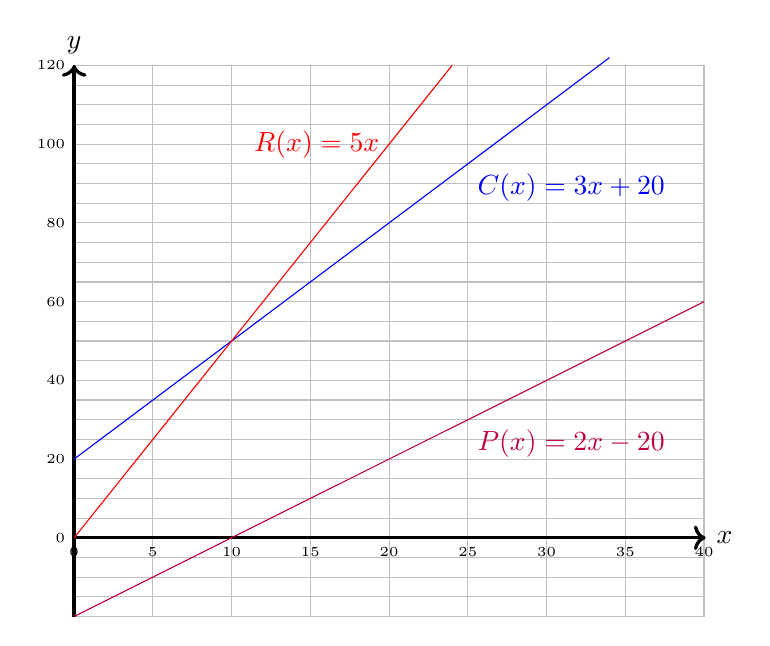
\begin{tikzpicture}[yscale=1/20, xscale=1/5]
    \draw[gray!50, thin, step=5] (0,-20) grid (40,120);
    \draw[very thick,->] (0,0) -- (40.1,0) node[right] {$x$};
    \draw[very thick,->] (0,-20) -- (0,120.1) node[above] {$y$};

    \foreach \x in {0,5,...,40} \draw (\x,0.05) -- (\x,-0.05) node[below] {\tiny\x};
    \foreach \y in {0,20,...,120} \draw (-0.05,\y) -- (0.05,\y) node[left] {\tiny\y};


    \draw[scale=1,domain=0:34,smooth,variable=\x,blue] plot ({\x},{3*\x+20});
  
    \draw[scale=1,domain=0:24,smooth,variable=\x,red] plot ({\x},{5*\x});

    \draw[scale=1,domain=0:40,smooth,variable=\x,purple] plot ({\x},{2*\x-20});

\draw[blue] (25,95) --node[below right]{$C(x)=3x+20$}(25,95);
\draw[red] (20,100) --node[left]{$R(x)=5x$}(20,100);
\draw[purple] (25,30) --node[below right]{$P(x)=2x-20$}(25,30);



\end{tikzpicture}$$ 

\url{https://www.desmos.com/calculator/d6l9b3kqho}

\item Since $P(x)=2x-20$, the change per unit of $x$ or profit per widget is the slope, or \$2/widget.

\item When you produce $\TCG{x=30}$ widgets, the cost will be:

\begin{eqnarray*}
C(x)&=&3x+20\\
C(x)&=&3\cdot\TCG{30}+20\\
C(x)&=&90+20\\
C(x)&=&110.\\
\end{eqnarray*}
The cost of producing 30 widgets is \$110.

 $$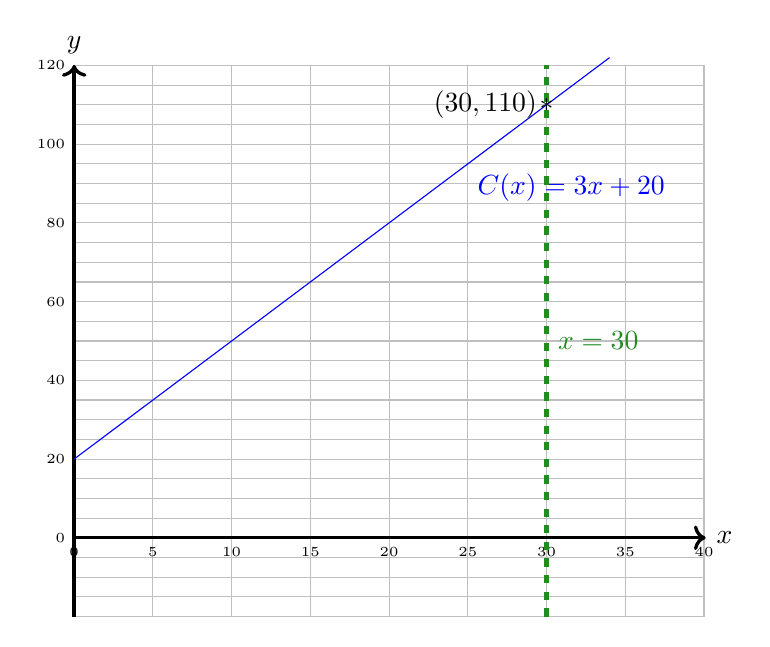
\begin{tikzpicture}[yscale=1/20, xscale=1/5]
    \draw[gray!50, thin, step=5] (0,-20) grid (40,120);
    \draw[very thick,->] (0,0) -- (40.1,0) node[right] {$x$};
    \draw[very thick,->] (0,-20) -- (0,120.1) node[above] {$y$};

    \foreach \x in {0,5,...,40} \draw (\x,0.05) -- (\x,-0.05) node[below] {\tiny\x};
    \foreach \y in {0,20,...,120} \draw (-0.05,\y) -- (0.05,\y) node[left] {\tiny\y};


    \draw[scale=1,domain=0:34,smooth,variable=\x,blue] plot ({\x},{3*\x+20});
  
%    \draw[scale=1,domain=0:24,smooth,variable=\x,red] plot ({\x},{5*\x});

%    \draw[scale=1,domain=0:40,smooth,variable=\x,purple] plot ({\x},{2*\x-20});

\draw[blue] (25,95) --node[below right]{$C(x)=3x+20$}(25,95);
%\draw[red] (20,100) --node[left]{$R(x)=5x$}(20,100);
%\draw[purple] (25,30) --node[below right]{$P(x)=2x-20$}(25,30);

\draw[ultra thick, dashed, ForestGreen] (30,-20) --node[right]{$x=30$} (30,120);

\node at (30,110){$*$};
\draw (30,110) --node[left]{$(30,110)$}(30,110);


\end{tikzpicture}$$ 
\url{https://www.desmos.com/calculator/cmoor2agyv}

\item The break even occurs when the profit is zero, $\TCO{P(x)=0}$.

\begin{eqnarray*}
P(x)&=&2x-20\\
\TCO{0}&=&2x-20\\
2x&=&20\\
x&=&10.
\end{eqnarray*}
The break even point occurs when $x=10$ widgets are sold.

 $$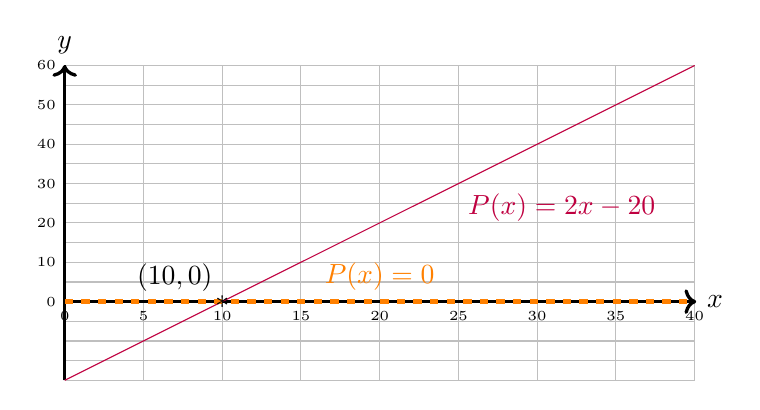
\begin{tikzpicture}[yscale=1/20, xscale=1/5]
    \draw[gray!50, thin, step=5] (0,-20) grid (40,60);
    \draw[very thick,->] (0,0) -- (40.1,0) node[right] {$x$};
    \draw[very thick,->] (0,-20) -- (0,60.1) node[above] {$y$};

    \foreach \x in {0,5,...,40} \draw (\x,0.05) -- (\x,-0.05) node[below] {\tiny\x};
    \foreach \y in {0,10,...,60} \draw (-0.05,\y) -- (0.05,\y) node[left] {\tiny\y};


%    \draw[scale=1,domain=0:34,smooth,variable=\x,blue] plot ({\x},{3*\x+20});
  
%    \draw[scale=1,domain=0:24,smooth,variable=\x,red] plot ({\x},{5*\x});

    \draw[scale=1,domain=0:40,smooth,variable=\x,purple] plot ({\x},{2*\x-20});

%\draw[blue] (25,95) --node[below right]{$C(x)=3x+20$}(25,95);
%\draw[red] (20,100) --node[left]{$R(x)=5x$}(20,100);
\draw[purple] (25,30) --node[below right]{$P(x)=2x-20$}(25,30);

\draw[ultra thick, dashed, orange] (0,0) --node[above]{$P(x)=0$} (40,0);

\node at (10,0){$*$};
\draw (10,0) --node[above left]{$(10,0)$}(10,0);


\end{tikzpicture}$$ 
\url{https://www.desmos.com/calculator/bdtdeqzqqa}

\end{enumerate}



\end{example}



\begin{example}
\Q Dr.\ Johnson is traveling to visit her mother for a holiday.  She drives at a constant speed of 75 mph.  After 3 hours, she passes a landmark that she knows is 200 miles from her mom's house.
\begin{enumerate}
    \item Find a function $D(t)$ that gives Dr.\ Johnson's distance to her mother house, in miles, after $t$ hours.
    \item How far away was she when she started driving?
    \item How many hours did it take from start to finish to complete this drive?
\end{enumerate}

\Sol 
\begin{enumerate}
    \item Since she is driving towards her mom's house, the distance from her to the house decreases at a rate of 75 miles per hour.  Thus $\TCR{m=-75}$.  At $t=3$ hours, her distance was 200 miles away.  Thus $\TCB{(3,200)}$ falls on the line representing this function.  Recall the techniques from Examples \ref{Example:PandS}, \ref{Example:PandSagain}.
     \begin{eqnarray*}
    D(t)&=&-75t+b\\
    \TCB{200}&=&\TCR{-75}\cdot\TCB{3}+b\\
    200&=&-225+b\\
    b&=&200+225=425.
    \end{eqnarray*}
    Thus $D(t)=-75t+425$.   
 $$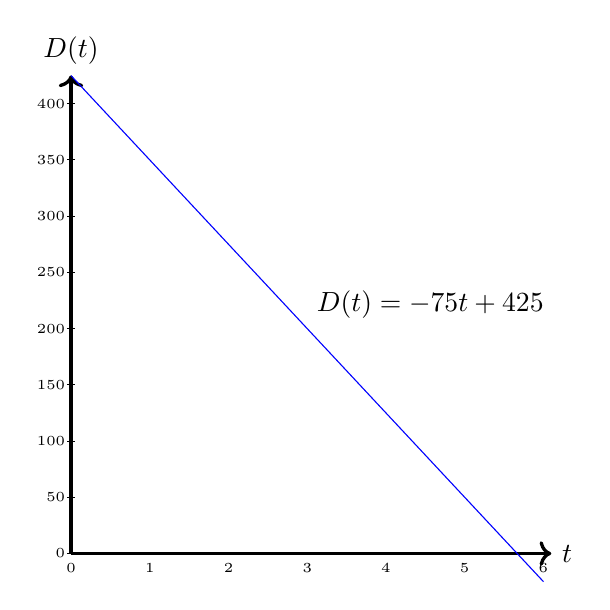
\begin{tikzpicture}[yscale=1/70]
    %\draw[gray!50, thin, step=5] (0,-20) grid (40,60);
    \draw[very thick,->] (0,0) -- (6.1,0) node[right] {$t$};
    \draw[very thick,->] (0,0) -- (0,425.1) node[above] {$D(t)$};

    \foreach \x in {0,1,...,6} \draw (\x,0.05) -- (\x,-0.05) node[below] {\tiny\x};
    \foreach \y in {0,50,...,425} \draw (-0.05,\y) -- (0.05,\y) node[left] {\tiny\y};



    \draw[scale=1,domain=0:6,smooth,variable=\x,blue] plot ({\x},{-75*\x+425});

\draw (3,200) --node[above right]{$D(t)=-75t+425$}(3,200);


%\node at (10,0){$*$};
%\draw (10,0) --node[above left]{$(10,0)$}(10,0);


\end{tikzpicture}$$ 
\url{https://www.desmos.com/calculator/uoul2cdsjs}
    \item At the start of the journey, $\TCG{t=0}$, and so she was $D(\TCG{0})=-75\cdot\TCG{0}+425=425$ miles from her mother's house.
\url{https://www.desmos.com/calculator/xuzh7xcgwk}    
    \item When she arrives, her distance from her mothers house is $\TCO{D(t)=0}$ miles and so:
     \begin{eqnarray*}
    D(t)&=&-75t+425\\
    \TCO{0}&=&-75t+425\\
    75t&=&425\\
    t&=&\frac{425}{75}\approx 5.6667.
    \end{eqnarray*}
So the trip takes $t=\frac{425}{75}\approx 5.6667$ hours or 5 hours and 40 minutes.    
 
$$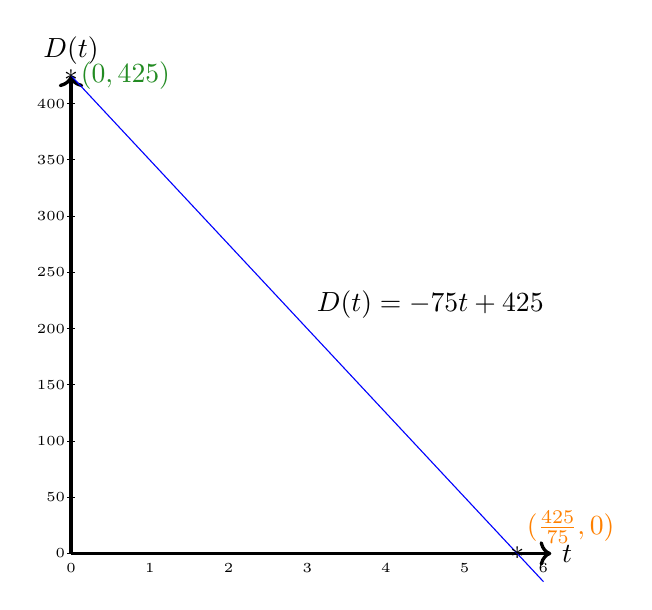
\begin{tikzpicture}[yscale=1/70]
    %\draw[gray!50, thin, step=5] (0,-20) grid (40,60);
    \draw[very thick,->] (0,0) -- (6.1,0) node[right] {$t$};
    \draw[very thick,->] (0,0) -- (0,425.1) node[above] {$D(t)$};

    \foreach \x in {0,1,...,6} \draw (\x,0.05) -- (\x,-0.05) node[below] {\tiny\x};
    \foreach \y in {0,50,...,425} \draw (-0.05,\y) -- (0.05,\y) node[left] {\tiny\y};



    \draw[scale=1,domain=0:6,smooth,variable=\x,blue] plot ({\x},{-75*\x+425});

\draw (3,200) --node[above right]{$D(t)=-75t+425$}(3,200);


\node at (0,425){$*$};
\draw[ForestGreen] (0,425) --node[right]{$(0,425)$}(0,425);

\node at (17/3,0){$*$};
\draw[orange] (17/3,0) --node[above right]{$(\frac{425}{75},0)$}(17/3,0);


\end{tikzpicture}$$  
 \url{https://www.desmos.com/calculator/dilrensiar}
    
\end{enumerate}


\end{example}


\begin{example}\label{Example:}
\Q Consider the following graphs of functions $q=S(p), D(p)$, where $p$ is the price of a product, and $q$ is the quantity demanded.

$$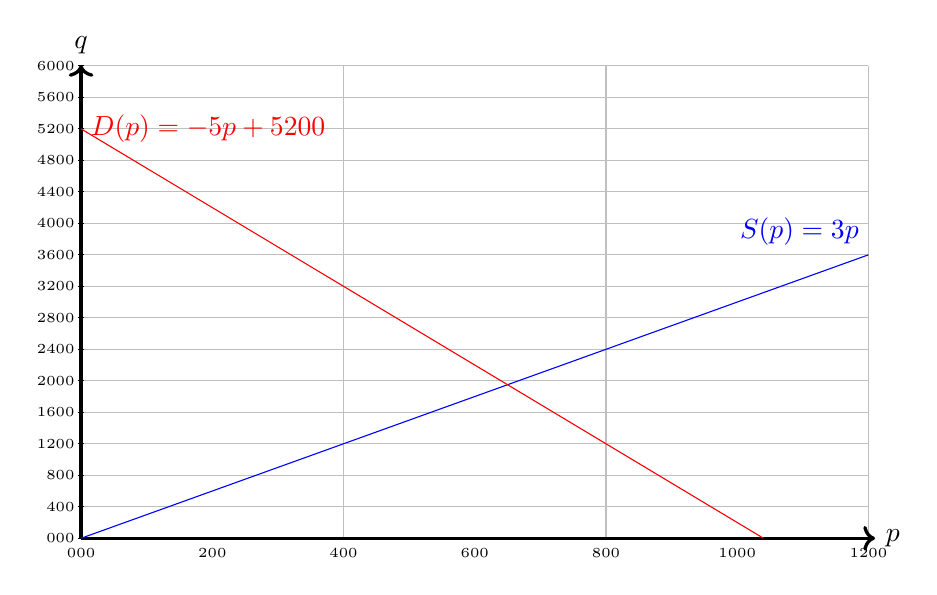
\begin{tikzpicture}[yscale=6/60, xscale=10/12]
    \draw[gray!50, thin, step=4] (0,0) grid (12,60);
    \draw[very thick,->] (0,0) -- (12.1,0) node[right] {$p$};
    \draw[very thick,->] (0,0) -- (0,60.1) node[above] {$q$};

    \foreach \x in {0,2,...,12} \draw (\x,0.05) -- (\x,-0.05) node[below] {\tiny\x00};
    \foreach \y in {0,4,...,60} \draw (-0.05,\y) -- (0.05,\y) node[left] {\tiny\y00};



    \draw[scale=1,domain=0:12,smooth,variable=\x,blue] plot ({\x},{3*\x});

    \draw[scale=1,domain=0:10.4,smooth,variable=\x,red] plot ({\x},{-5*\x+52});

\draw[red] (0,52) --node[right]{$D(p)=-5p+5200$}(0,52);
\draw[blue] (12,36) --node[above left]{$S(p)=3p$}(12,36);



\end{tikzpicture}$$

\begin{enumerate}
    \item Find the equations for the supply and demand curves $q=S(p), q=D(p)$, where $p$ is the price in dollars and $q$ is the quantity, either demanded or supplied.
    \item If \$350 is charged for this product, What is the surplus or deficit of products produced?
    \item Where is the equilibrium point (where supply and demand are the same)?
\end{enumerate}

\Sol

\begin{enumerate}
    \item It helps if we can identify some points on these lines.  We will work on them one at a time.
    \begin{enumerate}
        \item Graphically, we can see that $S(0)=0$, thus $(0,0)$ is on the supply line.  This also tells us the $q$-intercept, $b=0$.  We can also see that when $p=400, S(400)=1200$, thus $(400,1200)$ is also on this line.  Thus: $$m=\frac{1200-0}{400-0}=3.$$  So $S(p)=3p$.
        
        \item Graphically, we can see that $D(0)=5200$, thus $(0,5200)$ is on the demand line.  This also tells us the $q$-intercept, $b=5200$.  We can also see that when $p=400, D(400)=3200$, thus $(400,3200)$ is also on this line.  Thus: $$m=\frac{3200-5200}{400-0}=\frac{-2000}{400}=-5.$$  So $D(p)=-5p+5200$.
    \end{enumerate}
    \item When $p=350$, we will have $S(350)=3*350=1050$ products supplied, but $D(350)=-5*250+5200=3450$ demanded.  Thus there is a deficit of $3450-1050=2400$ products demanded that are not supplied, since demand exceeds supply.
    $$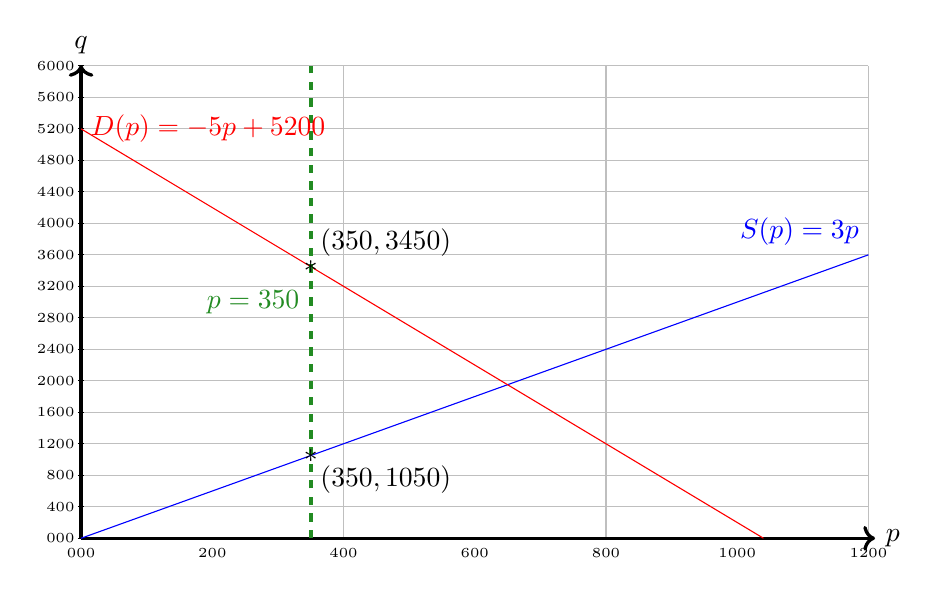
\begin{tikzpicture}[yscale=6/60, xscale=10/12]
    \draw[gray!50, thin, step=4] (0,0) grid (12,60);
    \draw[very thick,->] (0,0) -- (12.1,0) node[right] {$p$};
    \draw[very thick,->] (0,0) -- (0,60.1) node[above] {$q$};

    \foreach \x in {0,2,...,12} \draw (\x,0.05) -- (\x,-0.05) node[below] {\tiny\x00};
    \foreach \y in {0,4,...,60} \draw (-0.05,\y) -- (0.05,\y) node[left] {\tiny\y00};



    \draw[scale=1,domain=0:12,smooth,variable=\x,blue] plot ({\x},{3*\x});

    \draw[scale=1,domain=0:10.4,smooth,variable=\x,red] plot ({\x},{-5*\x+52});

    \draw[dashed, ultra thick, ForestGreen] (3.5,0) --node[left]{$p=350$} (3.5,60);

    \draw[red] (0,52) --node[right]{$D(p)=-5p+5200$}(0,52);
    \draw[blue] (12,36) --node[above left]{$S(p)=3p$}(12,36);
    
    \node at (3.5,34.5){$*$};
\draw (3.5,34.5) --node[above right]{$(350,3450)$}(3.5,34.5);

    \node at (3.5,10.5){$*$};
\draw (3.5,10.5) --node[below right]{$(350,1050)$}(3.5,10.5);


\end{tikzpicture}$$
\url{https://www.desmos.com/calculator/dee7rqh07j}

\item The equilibrium point is the point where the quantity supplied and demanded are the same.  Algebraically, this means $D(p)=S(p)$, and so:

\begin{eqnarray*}
-5p+5200&=&3p\\
5200&=&8p\\
p&=&\frac{5200}{8}=650.
\end{eqnarray*}

So the equilibrium happens when $p=650$ that is \$650 per unit.  Then, we note that $S(650)=3*650=1950$ and $D(p)=-5*650+5200=1950$, so the equilibrium point is $(650, 1950)$ or $\$650$ per unit, and 1950 units sold.

$$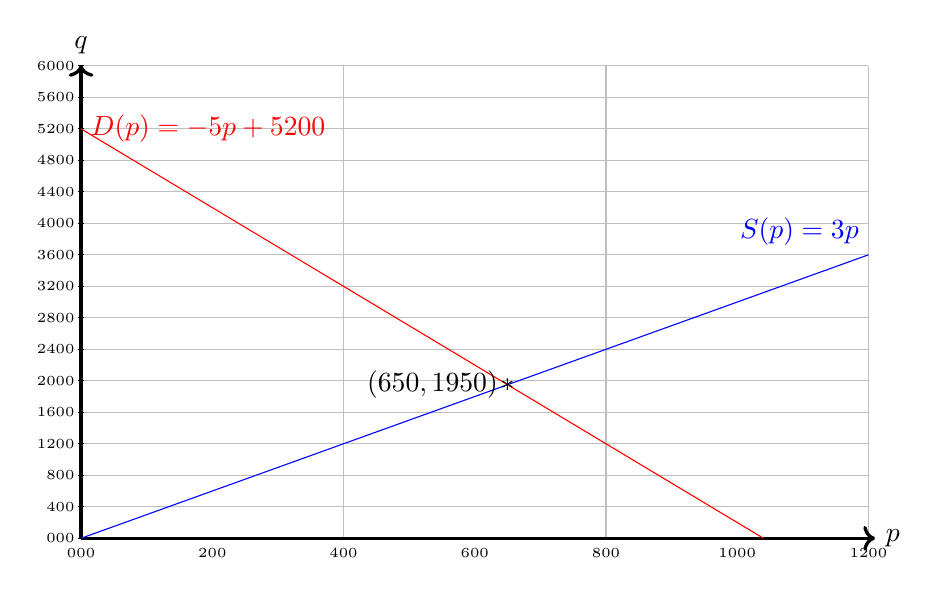
\begin{tikzpicture}[yscale=6/60, xscale=10/12]
    \draw[gray!50, thin, step=4] (0,0) grid (12,60);
    \draw[very thick,->] (0,0) -- (12.1,0) node[right] {$p$};
    \draw[very thick,->] (0,0) -- (0,60.1) node[above] {$q$};

    \foreach \x in {0,2,...,12} \draw (\x,0.05) -- (\x,-0.05) node[below] {\tiny\x00};
    \foreach \y in {0,4,...,60} \draw (-0.05,\y) -- (0.05,\y) node[left] {\tiny\y00};



    \draw[scale=1,domain=0:12,smooth,variable=\x,blue] plot ({\x},{3*\x});

    \draw[scale=1,domain=0:10.4,smooth,variable=\x,red] plot ({\x},{-5*\x+52});

\draw[red] (0,52) --node[right]{$D(p)=-5p+5200$}(0,52);
\draw[blue] (12,36) --node[above left]{$S(p)=3p$}(12,36);

    \node at (6.5,19.5){$*$};
\draw (6.5,19.5) --node[left]{$(650,1950)$}(6.5,19.5);



\end{tikzpicture}$$
\url{https://www.desmos.com/calculator/aywru3gvxu}
\end{enumerate}

\end{example}

These examples barely scratch the surface on how linear functions may be applied, but hopefully they gave you some sense on what sort of things they can be used to model, what sort of questions one can answer with them, and how to address them when the time comes.

\section{Linear Regression}


\subsection{Philosophy of Linear Regression}

It turns out that it's fairly rare to find variables in the world that are truly independent of each other.  The world is full of variables that have hidden connections and part of understanding the universe we exist in is uncovering all these connections.  This is true since the first cave person stood near a fire and realized that standing near a fire made them warmer, thus uncovering a connection between standing near fires and warmth.\\

However, since the world is an interconnected web of hidden influences, it's rare to see two variables that can be solely and completely determined by one another.  In the example of our erstwhile caveperson, it's certain that standing near fire could make you warm, but so could standing in sunlight, so could wearing more furs.  There are a lot of factors that go into determining warmth besides proximity to flames.\\

Our goal here then is to take observations and determine whether or not they are connected, and what the connection is so we could potentially use one as a predictor for the other.  But moreover, we also want to measure how strong this connection is so that we can asses how accurate these predictions might be, and what other variables may be influencing these outcomes.


\subsection{Basic Mechanics of Linear Regression}

Wee begin with an illustrative example.

\begin{example}\label{Example:BasicRegression}

\Q Consider the data set:

$$\begin{array}{c|c}
x&y\\
\hline
1&2\\
2&2\\
3&4\\
4&4\\
5&6
\end{array}$$


If we were to plot this data, it would look like:

$$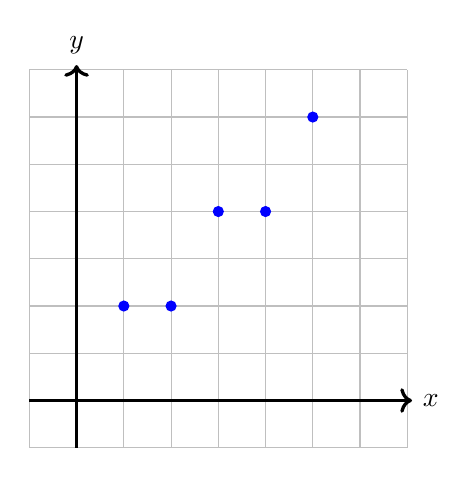
\begin{tikzpicture}[scale=.6][domain=-1:7]
    \draw[gray!50, thin, step=1] (-1,-1) grid (7,7);
    \draw[very thick,->] (-1,0) -- (7.1,0) node[right] {$x$};
    \draw[very thick,->] (0,-1) -- (0,7.1) node[above] {$y$};

%    \foreach \x in {-4,...,10} \draw (\x,0.05) -- (\x,-0.05) node[below] {\tiny\x};
%    \foreach \y in {-2,...,2} \draw (-0.05,\y) -- (0.05,\y) node[right] {\tiny\y};

\draw[blue, fill] (1,2) circle (3pt);
\draw[blue, fill] (2,2) circle (3pt);
\draw[blue, fill] (3,4) circle (3pt);
\draw[blue, fill] (4,4) circle (3pt);
\draw[blue, fill] (5,6) circle (3pt);

%  \draw[scale=1,domain=-2:2,smooth,variable=\x,blue] plot ({\x},{\x*\x*\x-3*\x}) node[above]{$y=f(x)$};


\end{tikzpicture}$$ % of mbox

Our goal here is to find a linear relationship between $x$ and $y$.  Graphically that means we want to draw a line that best fits the data we present here.  Of course, there is no line that can pass through all these points.  Our goal is to find the line that best fits these points, and to measure how well this line predicts actual values from the data.\\

\end{example}


We now commence with listing the basic arithmetic mechanics for finding a regression line.  Note that demonstrating why these formulations generate the best-fit line is beyond the scope of this text.  The most important thing to remember is: \\

``Given a bunch of points $(x_1, y_1), \ldots, (x_n, y_n)$, and a linear equation $\ell(x)=mx+b$ the \textbf{error} of each point is $e_i=\ell(x_i)-y_i$, that is the difference between the actual $y$ values, and what $\ell$ predicts should bee the $y$ values.  We are trying to find $m, b$ so that the sum of the errors squared $\sum e_i^2$ is minimized."\\

Why minimize $\sum e_i^2$?  Squaring the data erases the distinction between positive and negative error, between  over and under shoot.  Then, we want the total accumalated data to be as small as possible.




\begin{itemize}
\item $SS_X=\sum(x_i-\bar{x})^2=\sum x_i^2-\frac{(\sum x_i)^2}{n}$
\item $SS_Y=\sum(y_i-\bar{y})^2=\sum y_i^2-\frac{(\sum y_i)^2}{n}$
\item $SS_{XY}=\sum(x_i-\bar{x})(y_i-\bar{y})=\sum x_iy_i-\frac{(\sum x_i)(\sum y_i)}{n}$
\end{itemize}

The slope of the regression line will be:

$$\beta_1:=\frac{SS_{XY}}{SS_{X}}$$

If we recall, a line needs not just a slope, but a $y$ intercept.  So how can we figure out what the $y$ intercept should be?  Well, given the slope $\beta_1$, ON AVERAGE, given some $x_i$, we should get that $y_i=\beta_1x_i+\beta_0$, where $\beta_0$ is our yet-unknown $y$-intercept.  Again, this won't happen every time, or possibly ever, but it should be the average result, so the way we find $\beta_0$ is:

\begin{eqnarray*}
\bar{y}&=&\beta_1\bar{x}+\beta_0\\
\beta_0&=&\bar{y}-\beta_1\bar{x}.
\end{eqnarray*}

The above constructions are necessary to produce the best fit line.  In order to measure how good of a fit this line is, we introduce the \textbf{correlation coefficient}, usually denoted $r$.  This value is computed as follows:

$$r=\frac{n(\sum x_iy_i)-(\sum x_i)(\sum y_i)}{\sqrt{(n\sum x_i^2) - (\sum x_i)^2}\cdot \sqrt{n(\sum y_i^2)-(\sum y_i)^2}}.$$

This value measures the correction between the $x$ and $y$ values, with $r$ ranging from $-1$ to $1$.  The way we should interpret the $r$ values is as follows:

\begin{enumerate}
    \item Positive $r$ means positive correlation, meaning as $x$ goes up, $y$ tends to go up.  Negative $r$ means the opposite, as $x$ goes up, $y$ tends to go down.  Correlation of 0 means $x$'s change does not predict whether or not $y$ goes up or down.
    
    \item The closer $r$ is to 0, the weaker the correlation, meaning the ability to predict $y$ from $x$ is weak, the closer to $-1$ or $1$, the better our ability to predict $y$ from $x$.
\end{enumerate}

\begin{example}\label{Example:visualizecorr}
Consider the following plots of points.  Whether the points tend to have an upward or downward trend determines the sign of $r$, how well the best fit line predicts the points determines how close $r$ is to either $-1$ or $1$.

$$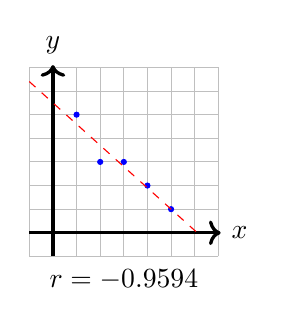
\begin{tikzpicture}[scale=.3][domain=-1:7]
    \draw[gray!50, thin, step=1] (-1,-1) grid (7,7);
    \draw[very thick,->] (-1,0) -- (7.1,0) node[right] {$x$};
    \draw[very thick,->] (0,-1) -- (0,7.1) node[above] {$y$};

%    \foreach \x in {-4,...,10} \draw (\x,0.05) -- (\x,-0.05) node[below] {\tiny\x};
%    \foreach \y in {-2,...,2} \draw (-0.05,\y) -- (0.05,\y) node[right] {\tiny\y};

\draw[blue, fill] (1,5) circle (3pt);
\draw[blue, fill] (2,3) circle (3pt);
\draw[blue, fill] (3,3) circle (3pt);
\draw[blue, fill] (4,2) circle (3pt);
\draw[blue, fill] (5,1) circle (3pt);

  \draw[scale=1,domain=-1:6.111,smooth,variable=\x,red, dashed] plot ({\x},{-0.9*\x+5.5});

\draw (3, -2) --node{$r=-0.9594$} (3,-2);

\end{tikzpicture}
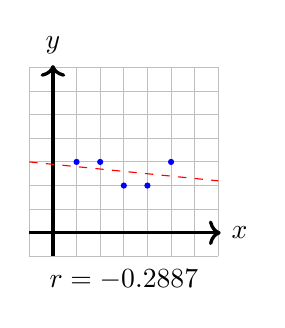
\begin{tikzpicture}[scale=.3][domain=-1:7]
    \draw[gray!50, thin, step=1] (-1,-1) grid (7,7);
    \draw[very thick,->] (-1,0) -- (7.1,0) node[right] {$x$};
    \draw[very thick,->] (0,-1) -- (0,7.1) node[above] {$y$};

%    \foreach \x in {-4,...,10} \draw (\x,0.05) -- (\x,-0.05) node[below] {\tiny\x};
%    \foreach \y in {-2,...,2} \draw (-0.05,\y) -- (0.05,\y) node[right] {\tiny\y};

\draw[blue, fill] (1,3) circle (3pt);
\draw[blue, fill] (2,3) circle (3pt);
\draw[blue, fill] (3,2) circle (3pt);
\draw[blue, fill] (4,2) circle (3pt);
\draw[blue, fill] (5,3) circle (3pt);

  \draw[scale=1,domain=-1:7,smooth,variable=\x,red, dashed] plot ({\x},{-0.1*\x+2.9});

\draw (3, -2) --node{$r=-0.2887$} (3,-2);

\end{tikzpicture}
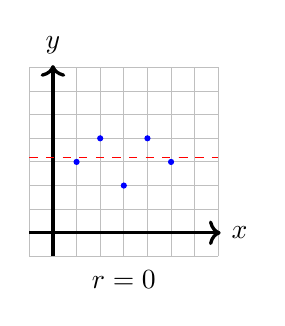
\begin{tikzpicture}[scale=.3][domain=-1:7]
    \draw[gray!50, thin, step=1] (-1,-1) grid (7,7);
    \draw[very thick,->] (-1,0) -- (7.1,0) node[right] {$x$};
    \draw[very thick,->] (0,-1) -- (0,7.1) node[above] {$y$};

%    \foreach \x in {-4,...,10} \draw (\x,0.05) -- (\x,-0.05) node[below] {\tiny\x};
%    \foreach \y in {-2,...,2} \draw (-0.05,\y) -- (0.05,\y) node[right] {\tiny\y};

\draw[blue, fill] (1,3) circle (3pt);
\draw[blue, fill] (2,4) circle (3pt);
\draw[blue, fill] (3,2) circle (3pt);
\draw[blue, fill] (4,4) circle (3pt);
\draw[blue, fill] (5,3) circle (3pt);

  \draw[scale=1,domain=-1:7,smooth,variable=\x,red, dashed] plot ({\x},{3.2});

\draw (3, -2) --node{$r=0$} (3,-2);

\end{tikzpicture}
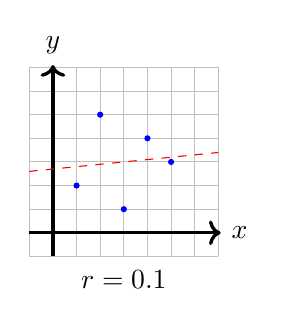
\begin{tikzpicture}[scale=.3][domain=-1:7]
    \draw[gray!50, thin, step=1] (-1,-1) grid (7,7);
    \draw[very thick,->] (-1,0) -- (7.1,0) node[right] {$x$};
    \draw[very thick,->] (0,-1) -- (0,7.1) node[above] {$y$};

%    \foreach \x in {-4,...,10} \draw (\x,0.05) -- (\x,-0.05) node[below] {\tiny\x};
%    \foreach \y in {-2,...,2} \draw (-0.05,\y) -- (0.05,\y) node[right] {\tiny\y};

\draw[blue, fill] (1,2) circle (3pt);
\draw[blue, fill] (2,5) circle (3pt);
\draw[blue, fill] (3,1) circle (3pt);
\draw[blue, fill] (4,4) circle (3pt);
\draw[blue, fill] (5,3) circle (3pt);

  \draw[scale=1,domain=-1:7,smooth,variable=\x,red, dashed] plot ({\x},{0.1*\x+2.7});

\draw (3, -2) --node{$r=0.1$} (3,-2);

\end{tikzpicture}
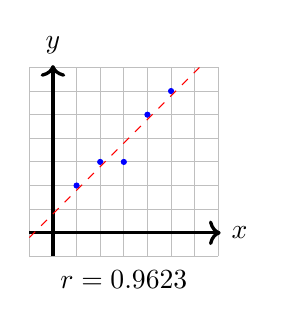
\begin{tikzpicture}[scale=.3][domain=-1:7]
    \draw[gray!50, thin, step=1] (-1,-1) grid (7,7);
    \draw[very thick,->] (-1,0) -- (7.1,0) node[right] {$x$};
    \draw[very thick,->] (0,-1) -- (0,7.1) node[above] {$y$};

%    \foreach \x in {-4,...,10} \draw (\x,0.05) -- (\x,-0.05) node[below] {\tiny\x};
%    \foreach \y in {-2,...,2} \draw (-0.05,\y) -- (0.05,\y) node[right] {\tiny\y};

\draw[blue, fill] (1,2) circle (3pt);
\draw[blue, fill] (2,3) circle (3pt);
\draw[blue, fill] (3,3) circle (3pt);
\draw[blue, fill] (4,5) circle (3pt);
\draw[blue, fill] (5,6) circle (3pt);

  \draw[scale=1,domain=-1:6.2,smooth,variable=\x,red, dashed] plot ({\x},{\x+0.8});

\draw (3, -2) --node{$r=0.9623$} (3,-2);

\end{tikzpicture}
$$
$$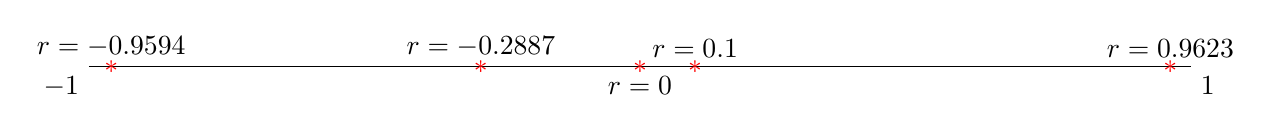
\begin{tikzpicture}[scale=7]
    \draw (-1,0)--(1,0);
    \draw (-1,0)--node[below left]{$-1$}(-1,0);
    \draw (1,0)--node[below right]{$1$}(1,0);  
    \draw[red]( 0.9623,0)--node{$*$}( 0.9623,0);
    \draw( 0.9623,0)--node[above]{$r=0.9623$}( 0.9623,0);
    \draw[red]( 0.1,0)--node{$*$}( 0.1,0);
    \draw( 0.1,0)--node[above]{$r=0.1$}( 0.1,0);
    \draw[red]( 0.0,0)--node{$*$}( 0.0,0);
    \draw( 0.0,0)--node[below]{$r=0$}( 0.0,0);
     \draw[red]( -0.2887,0)--node{$*$}( -0.2887,0);
    \draw( -0.2887,0)--node[above]{$r=-0.2887$}( -0.2887,0);
     \draw[red]( -0.9594,0)--node{$*$}( -0.9594,0);
    \draw( -0.9594,0)--node[above]{$r=-0.9594$}( -0.9594,0);
\end{tikzpicture}
$$
\end{example}

We further note that the closer $r$ is to either $-1, 1$ the closer $r^2$ is to 1, and similarly the closer $r$ is to 0, the closer $r^2$ is to 1.  Thus, we use $r^2$ as an overall measure of the strength of the correlation.  In fact, we say that $y$ is $r^2$ predicted by $x$, that is the values of $y$ are $r^2$ determinable by the values of $x$, the rest by other, as of yet undetermined variables.



\begin{example}\label{Example:BasicRegressionContd}
We continue from Example \ref{Example:BasicRegression}:

\begin{eqnarray*}
\bar{x}&=&\frac{1+2+3+4+5}{5}=3\\
\bar{y}&=&\frac{2+2+4+4+6}{5}=3.6\\
SS_X&=&(1-3)^2+(2-3)^2+(3-3)^2+(4-3)^2+(5-3)^2=10\\
SS_Y&=&(2-3.5)^2+(2-3.5)^2+(4-3.5)^2+(4-3.5)^2+(6-3.5)^2=11.25\\
SS_{XY}&=&(1-3)(2-3.5)+(2-3)(2-3.5)+(3-3)(4-3.5)+\\
&&(4-3)(4-3.5)+(5-3)(6-3.5)=10\\
\beta_1&=&\frac{10}{10}=1\\
\beta_0&=&3.6-(1)(3)=0.6
\end{eqnarray*}

So our best fit line is $y=1x+0.6$.



$$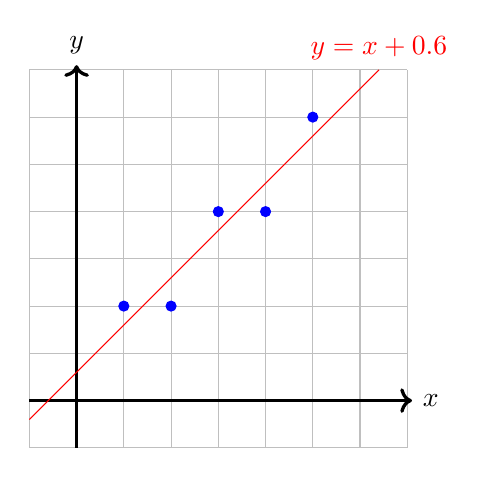
\begin{tikzpicture}[scale=.6][domain=-1:7]
    \draw[gray!50, thin, step=1] (-1,-1) grid (7,7);
    \draw[very thick,->] (-1,0) -- (7.1,0) node[right] {$x$};
    \draw[very thick,->] (0,-1) -- (0,7.1) node[above] {$y$};

%    \foreach \x in {-4,...,10} \draw (\x,0.05) -- (\x,-0.05) node[below] {\tiny\x};
%    \foreach \y in {-2,...,2} \draw (-0.05,\y) -- (0.05,\y) node[right] {\tiny\y};

\draw[blue, fill] (1,2) circle (3pt);
\draw[blue, fill] (2,2) circle (3pt);
\draw[blue, fill] (3,4) circle (3pt);
\draw[blue, fill] (4,4) circle (3pt);
\draw[blue, fill] (5,6) circle (3pt);

  \draw[scale=1,domain=-1:6.4,smooth,variable=\x,red] plot ({\x},{\x+0.6}) node[above]{$y=x+0.6$};


\end{tikzpicture}$$

Again, notice that none of the points actually fall on this line, but no possible line could have accomplished all of the points falling on it.  What we have instead is a line that passes through the points as closely as possible.  Define $e_i$ to be the error in prediction for $y_i$, that is let $e_i=y_i-(1\cdot x_i+0.6)$, then we see that:

\begin{eqnarray*}
e_1&=&2-(1+.6)=0.4\\
e_2&=&2-(2+.6)=-0.6\\
e_3&=&4-(3+.6)=0.4\\
e_4&=&4-(4+.6)=-0.6\\
e_5&=&6-(5+.6)=0.4
\end{eqnarray*}

$$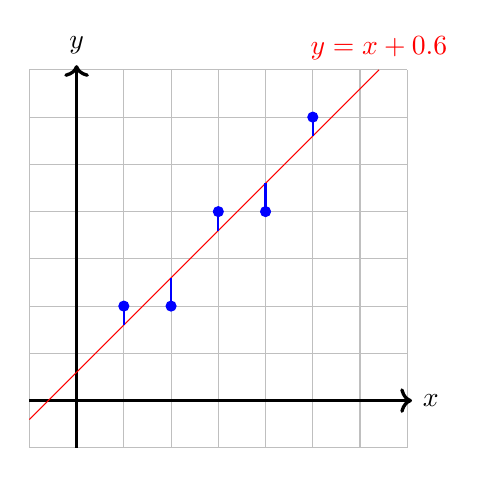
\begin{tikzpicture}[scale=.6][domain=-1:7]
    \draw[gray!50, thin, step=1] (-1,-1) grid (7,7);
    \draw[very thick,->] (-1,0) -- (7.1,0) node[right] {$x$};
    \draw[very thick,->] (0,-1) -- (0,7.1) node[above] {$y$};

%    \foreach \x in {-4,...,10} \draw (\x,0.05) -- (\x,-0.05) node[below] {\tiny\x};
%    \foreach \y in {-2,...,2} \draw (-0.05,\y) -- (0.05,\y) node[right] {\tiny\y};

\draw[blue, fill] (1,2) circle (3pt);
\draw[blue, fill] (2,2) circle (3pt);
\draw[blue, fill] (3,4) circle (3pt);
\draw[blue, fill] (4,4) circle (3pt);
\draw[blue, fill] (5,6) circle (3pt);

  \draw[scale=1,domain=-1:6.4,smooth,variable=\x,red] plot ({\x},{\x+0.6}) node[above]{$y=x+0.6$};

\draw[blue, thick](1, 1.6) -- (1,2);
\draw[blue, thick](2, 2.6) -- (2,2);
\draw[blue, thick](3, 3.6) -- (3,4);
\draw[blue, thick](4, 4.6) -- (4,4);
\draw[blue, thick](5, 5.6) -- (5,6);


\end{tikzpicture}$$


But $$e_1+e_2+e_3+e_4+e_5=(0.4)+(-0.6)+(0.4)+(0.6)+(0.4)=0.$$

This tells us this line passes through the ``middle" of the points.  Is it the best possible line?  Notice that $$\sum e_i^2=(0.4)^2+(-0.6)^2+(0.4)^2+(0.6)^2+(0.4)^2=1.2.$$  Is this the best we can do?  Again, a formal verification of this is beyond this text, but following this link: \url{https://www.desmos.com/calculator/gruczlkyyf}, you can see that by adjusting the parameters $m$ and $b$, that the sum of squares being 1.2 is the smallest error sum you can achieve.\\

To find $r$ we note that:

\begin{eqnarray*}
r&=&\frac{n(\sum x_iy_i)-(\sum x_i)(\sum y_i)}{\sqrt{(n\sum x_i^2) - (\sum x_i)^2}\cdot \sqrt{n(\sum y_i^2)-(\sum y_i)^2}}\\
&=&\frac{5(64)-(15)(18)}{\sqrt{5(55) - (15)^2}\cdot \sqrt{5(76)-(18)^2}}\\
&\approx&0.9449.
\end{eqnarray*}
So we can see that this fit is fairly close, and $x$ is a good predictor of $y$.  Since $r^2\approx 0.8929$, we can say that $y$'s value are 89.29\% determinable by $x$'s values.
\end{example}

\subsection{Good thing we don't live in the stone age.}

We should all agree that this was quite a lot of work to find these parameters for 5 values, and most data sets of work, have dozens, if not hundreds or thousands of data points.  It's simply impractical to do this by hand.\\

On the other hand a quick use of Desmos: \url{https://www.desmos.com/calculator/ir10f1wwzr} and entering the data points into the table, produces the best fit line, a plot, and the correlation coefficients.\\

Try entering your own data, adding or removing rows, and see how quickly and readily it will obtain our best fit lines and correlation coefficients!



\subsection{Applications}

\begin{example}
From fbi.gov from 2004-2013, the murder rates per 100,000 people are listed below:

$$\begin{array}{c|c}
\text{Years after 2000} & \text{Murders per 100,000 people}\\
x&y\\
\hline
4&5.5\\
5&5.6\\
6&5.8\\
7&5.7\\
8&5.4\\
9&5\\
10&4.8\\
11&4.7\\
12&4.7\\
13&4.5
\end{array}$$
\begin{enumerate}
\item Determine the best fit line for murders (per 100,000 people) $x$ years after 2000.
\item How much of a factor is the year in predictiung the number of murders?
\item Predict the murder rate in 2018.
\end{enumerate}

Entering this data in desmos: \url{https://www.desmos.com/calculator/em6xkq7udn}

\begin{enumerate}
\item It seems that the best fit line is $y=-0.144848x+6.40121$.
\item Since $r^2=0.8318$, we can say the murder rate is 83.18\% predictable by the year.
\item In 2018, the murder rate should be $-0.144848(18)+6.40121=3.793946$ or roughly 3.8 murders per 100,000 people in 2018.
\end{enumerate}




\end{example}



\begin{example}\label{Example:CorrQuizTest}
I personally wondered in quiz scores are a good predictor of test scores in Calculus.  I pulled out some data from this semester, and here are the average quiz and test scores of my students, anonymously of course:


$$\begin{array}{c|c}
\text{Quiz Average} & \text{Test Average}\\
x&y\\
\hline
87.5&100\\
76.13&94\\
75.83&93.5\\
53.53&83.5\\
76.13&83\\
71.13&78.85\\
56.13&76.5\\
73.57&70\\
66.13&69.5\\
66.13&63
\end{array}$$



\end{example}
\begin{enumerate}
\item Find the linear relationship between Quiz grades and Test grades.
\item Are Quiz grades a good predictor of Test grades?
\item If someone has an 80 average on Quizzes, predict their Test grade.
\end{enumerate}

So, once again:  \url{https://www.desmos.com/calculator/atipunytb1}

\begin{enumerate}
\item The relationship here is: $y=0.639883x+36.2168$, so there is a positive correlation, which we expect.
\item $r^2=0.2906$, so Test grades 29.06\% predictable by Quiz grades, which one would also expect, some people perform better in the Exam situation and some people perform worse.
\item We would have an expected test grade of $y=0.639883(80)+36.2168=87.40744$ or about 87.41\%.  But of course with an $r^2$ that small we shouldn't expect this to be terribly accurate.
\end{enumerate}


\subsection{Correlation $\neq$ Causation!}

A common misconception about correlated variables is that a strong correlation means that the $x$ variables \textbf{causes} the $y$ variable.  This is sometimes the case, but very often not true.\\

It is just as possible that $y$ causes $x$, or that $x$ and $y$ \textbf{share} common causes, or there's always complete coincidence.\\

In Example \ref{Example:CorrQuizTest}, if I had simply given everyone 100 on the quizzes without looking at them, and graded the exams in normal way, they likely would not have done any better.  One could argue that they would have done worse as a result.  So a positive correlation between the variables doesn't mean that one will rise simply by virtue of the other rising.\\

The bottom line is that correlations measure the strength and form of a relationship between variables, but not the nature of the relationship.











\chapter{Systems of Linear Equations and Matrices}\label{Chapter:Matrices}


\section*{Introduction}

In this chapter, we introduce the notion of Linear Systems.  Linear Systems occur whenever we have collections of variables with linear relations with each other.  For example, we may want to eat a diet which contains certain levels of protein and fiber, and we wonder how much chicken and kale we should eat to achieve this?  Or we have Business, English and Math students, each of whom take different number of these courses, if we knew how many of each major there were, could we compute how many credits of each type of course would be taught?  This chapter will focus on the techniques and tools to model and address these types of situations.



\section{Systems of Linear  Equations}\label{Section:SystemsofEquations}

A system of equations with unknowns $x_1,\ldots,x_n$ is a collection of first degree equations:

\begin{eqnarray*}
a_{1,1}x_1+a_{1,2}x_2+\cdots+a_{1,n}x_n&=&b_1\\
a_{2,1}x_1+a_{2,2}x_2+\cdots+a_{2,n}x_n&=&b_1\\
\vdots &=&\vdots\\
a_{m,1}x_1+a_{m,2}x_2+\cdots+a_{m,n}x_n&=&b_1\\
\end{eqnarray*}



\subsection{What Exactly is  a Solution to a System of Linear Equations?}

To answer the question that is the name of this section, we should kinda back up here and ask ``What is a solution to an equation?"\\

For example, what is a solution to $y=2x+3$? After dealing with linear equations in Chapter 1, we should have some sense as to what $y=2x+3$ looks like, that is a line with slope 2 and $y$-intercept $(0,3)$.  But what IS this line?  It's the collection of all points $(x,y)$ that make the above equation true.  So $(0,3), (-1,1)$ and $(2,7)$ are all on this line because they make the equation true ($3=2(0)+3, 1=2(-1)+3, 7=2(2)+3$).  A point like $(1,1)$ is NOT on this line because $1\neq 2(1)+3$.  \\

So a solution to an equation is \textbf{any point which makes the equation true}.\\

A \textit{System of Equations} is a collection of equations.  Thus, a solution to a system of equations is \textbf{any point which makes \underline{all} the equations true}.

\subsection{What are the Types of Solutions that we can have?}

So a solution to the system:

\begin{eqnarray*}
2x+3y&=&15\\
x-y&=&0
\end{eqnarray*}
is a collection of points that satisfy the first AND the second linear equalities.  The first equation describes the line: $y=-\frac{2}{3}x+5$, whereas the second describes the line $y=x$.  Each of these equations represent lines, so each individually has infinitely many solutions.  The question is, how many solutions do these lines have in common?\\

There are a number of ways to find out, but the most straight forward is simply to graph the system:

$$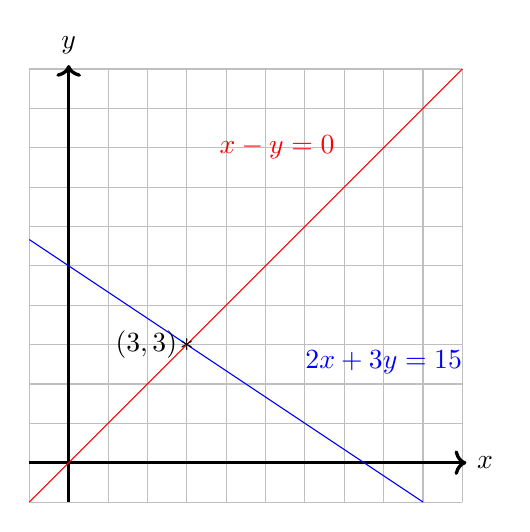
\begin{tikzpicture}[scale=0.5][domain=-1:10]
    \draw[gray!50, thin, step=1] (-1,-1) grid (10,10);
    \draw[very thick,->] (-1,0) -- (10.1,0) node[right] {$x$};
    \draw[very thick,->] (0,-1) -- (0,10.1) node[above] {$y$};

%    \foreach \x in {0,...,11} \draw (\x,0.05) -- (\x,-0.05) node[below] {\tiny\x};
%    \foreach \y in {0,...,28} \draw (-0.05,\y) -- (0.05,\y) node[right] {\tiny\y};


    \draw[scale=1,domain=-1:9,smooth,variable=\x,blue] plot ({\x},{(-2/3)*\x+5});
   \draw[scale=1,domain=-1:10,smooth,variable=\x,red] plot ({\x},{\x});

\node at (3,3){$*$};
\draw (3,3) --node[left]{$(3,3)$}(3,3);
\draw[blue] (8,2) --node[above]{$2x+3y=15$}(8,2);
\draw[red] (7,8) --node[left]{$x-y=0$}(7,8);



\end{tikzpicture}$$   


\url{https://www.desmos.com/calculator/cdrgyxm2al}.

As one can see, although each line has infinitely many points, the only solution they have in common is the point $(3,3)$.  To verify this, we note that $2(3)+3(3)=15$ and $3-3=0$, so both equations are satisfied.  This system has \textbf{a unique solution}\\

What else could happen when solving a system of equations?  Well, consider:


\begin{eqnarray*}
x+y&=&5\\
2x+2y&=&10.
\end{eqnarray*}

If we look at the graph of both lines, we only see one actual line:
 $$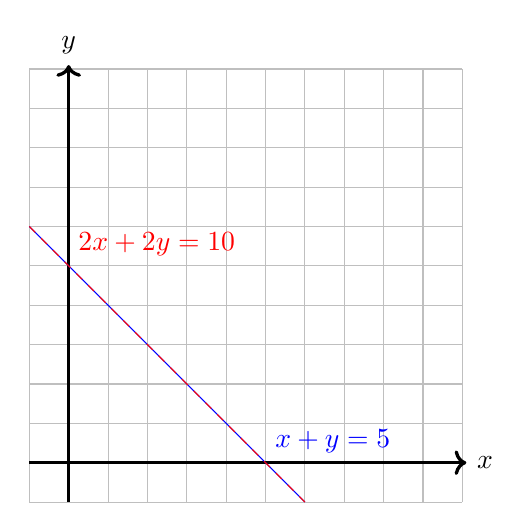
\begin{tikzpicture}[scale=0.5][domain=-1:10]
    \draw[gray!50, thin, step=1] (-1,-1) grid (10,10);
    \draw[very thick,->] (-1,0) -- (10.1,0) node[right] {$x$};
    \draw[very thick,->] (0,-1) -- (0,10.1) node[above] {$y$};

%    \foreach \x in {0,...,11} \draw (\x,0.05) -- (\x,-0.05) node[below] {\tiny\x};
%    \foreach \y in {0,...,28} \draw (-0.05,\y) -- (0.05,\y) node[right] {\tiny\y};


    \draw[scale=1,domain=-1:6,smooth,variable=\x,blue] plot ({\x},{(-1)*\x+5});
   \draw[scale=1,domain=-1:6,smooth,variable=\x,red, dashed] plot ({\x},{-1*\x+5});


\draw[blue] (5,0) --node[above right]{$x+y=5$}(5,0);
\draw[red] (0,5) --node[above right]{$2x+2y=10$}(0,5);


\end{tikzpicture}$$   


\url{https://www.desmos.com/calculator/oaqbrkruhl}. 

This is because both equations describe the same line.  After all, whenever $x+y=5$, it would have to be true that $2(x+y)=5\cdot2$ and thus $2x+2y=10$.  So ANY point that is a solution to one equation is a solution to the other, this system has \textbf{infinitely many solutions}.\\

Another possibility arises from the following example:


\begin{eqnarray*}
x+y&=&5\\
x+y&=&6\end{eqnarray*}

If we graph these lines side by side:

$$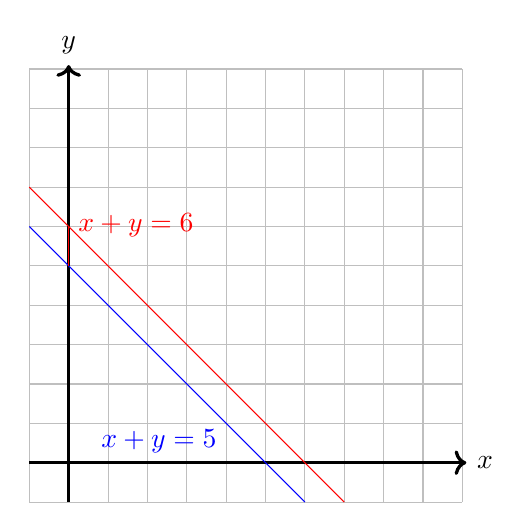
\begin{tikzpicture}[scale=0.5][domain=-1:10]
    \draw[gray!50, thin, step=1] (-1,-1) grid (10,10);
    \draw[very thick,->] (-1,0) -- (10.1,0) node[right] {$x$};
    \draw[very thick,->] (0,-1) -- (0,10.1) node[above] {$y$};

%    \foreach \x in {0,...,11} \draw (\x,0.05) -- (\x,-0.05) node[below] {\tiny\x};
%    \foreach \y in {0,...,28} \draw (-0.05,\y) -- (0.05,\y) node[right] {\tiny\y};


    \draw[scale=1,domain=-1:6,smooth,variable=\x,blue] plot ({\x},{(-1)*\x+5});
   \draw[scale=1,domain=-1:7,smooth,variable=\x,red] plot ({\x},{-1*\x+6});


\draw[blue] (4,0) --node[above left]{$x+y=5$}(4,0);
\draw[red] (0,6) --node[above right]{$x+y=6$}(0,5);


\end{tikzpicture}$$   


\url{https://www.desmos.com/calculator/djqxxge4ce}. 

We can see that these lines are parallel and do not actually have any points in common.  After all, how many pairs of numbers $x$ and $y$ sum to both 5 AND 6?  It should be clear that this system has \textbf{no solutions}.\\

Of course, these have all been Systems of Linear Equations in 2 variables.  When we increase the number of variables, we increase the dimensionality of the potential solution space, and what it means to be ``linear" changes somewhat.  Nevertheless, these examples illustrate the 3 possible outcomes of a system of linear equations in any dimension:

\begin{itemize}
\item There is a unique Solution.
\item There are infinitely many Solutions.
\item There are no Solutions.
\end{itemize}



\subsection{How do we find the Solution(s)/know we have No Solutions?}

In 2 variables, it's simple enough we can just graph, as we did above.  But we should try to develop some algebraic techniques as well, since this will be harder to do when we increase the dimensions of our problems.\\


What we introduce here is the Echelon Method, the general goal is to take non-zero multiples of our equations and use them to eliminate variables in the other equations so that a solution to a variable can be made known.  This process should also reveal if there are infinitely many or no solutions.\\


\begin{example}
\begin{eqnarray*}
2x+3y&=&1\\
x+y&=&0
\end{eqnarray*}

We note that whatever the solutions to this are, they should be the same as the solutions to:

\begin{eqnarray*}
x+\frac{3}{2}y&=&\frac{1}{2}\\
x+y&=&0
\end{eqnarray*}

We've divided the first equation in half, but we haven't actually changed what points will make that equation true.  Then:

\begin{eqnarray*}
x+\frac{3}{2}y&=&\frac{1}{2}\\
x+y-(x+\frac{3}{2}y)&=&0-\frac{1}{2}
\end{eqnarray*}

Must also be true, since we can add and subtract the same values from 2 sides of an equation and preserve the solutions.  By doing this, we kill off the $x$ in the second equation and we can solve for $y$:

\begin{eqnarray*}
x+\frac{3}{2}y&=&\frac{1}{2}\\
-\frac{1}{2}y&=&-\frac{1}{2}
\end{eqnarray*}

So $y=1$ based on the second line.  

\begin{eqnarray*}
x+\frac{3}{2}y&=&\frac{1}{2}\\
y&=&1
\end{eqnarray*}


If we take $-\frac{3}{2}$ times the second line and add it to the first:

\begin{eqnarray*}
x+\frac{3}{2}y-\frac{3}{2}(y)&=&\frac{1}{2}-\frac{3}{2}(1)\\
y&=&1
\end{eqnarray*}

We obtain:

\begin{eqnarray*}
x&=&-1\\
y&=&1
\end{eqnarray*}

We can verify that if we consider the original system:


\begin{eqnarray*}
2x+3y&=&1\\
x+y&=&0
\end{eqnarray*}
 then by evaluating at $x=-1, y=1$:
 
\begin{eqnarray*}
2(-1)+3(1)=-2+3&=&1\\
-1+1&=&0
\end{eqnarray*}
 


\end{example}

\begin{example} So if we consider:

\begin{eqnarray*}
x+y&=&2\\
2x+2y&=&4.
\end{eqnarray*}

Just like before, we want to kill the $x$ in the second equation:

\begin{eqnarray*}
x+y&=&2\\
2x+2y-2(x+y)&=&4-2(2).
\end{eqnarray*}

Which gives us:

\begin{eqnarray*}
x+y&=&2\\
0&=&0.
\end{eqnarray*}

Well..., certainly that second line doesn't contribute much, zero is always equal to itself.  So the solutions are just whenever $x+y=2$, which happens for infinitely many possible pairs.


\end{example}

\begin{example}


 Lastly, when we look at:

\begin{eqnarray*}
x+y&=&0\\
x+y&=&1.
\end{eqnarray*}

We can try to kill the $x$ in the second line as before:

\begin{eqnarray*}
x+y&=&0\\
x+y-(x+y)&=&1-0.
\end{eqnarray*}

Where we get:

\begin{eqnarray*}
x+y&=&0\\
0&=&1.
\end{eqnarray*}

So all you have to do is find a pair $(x,y)$ so that $0=1$... which is not ever going to happen.  So this will never have a solution.


\end{example}



\section{Representing a System of Linear Equations as a Matrix}\label{Section:SystemasMatrix}

Given a system of equations, we can try to encode that information in a matrix:

So for example the system of equations:

\begin{eqnarray*}
2x+3y+z&=&3\\
-2x+4y+2z&=&0\\
x-y+2z&=&3
\end{eqnarray*}

Would have matrix representation:

$$ \left( \begin{array}{rrr|r}
2 & 3 & 1& 3\\
-2 & 4 & 2 & 0\\
1 & -1 & 2 & 3
\end{array}\right).$$

A \textbf{matrix} is a rectangular array of numbers, each number is an \textbf{entry} of the matrix.  In the above example, the vertical line is a visual reminder to separate the constant terms from the variables.  A matrix displayed this way is an \textbf{augmented matrix}.

By letting each column of a matrix represent a different variable or constant and arranging the linear equations into rows, one can write any linear system of equations as an augmented matrix.   Conversely, if you have a matrix:

$$ \left( \begin{array}{rr|r}
1 & 2 & 4\\
3 & 3  & 9\\
\end{array}\right)$$

This represent the system of equations:


\begin{eqnarray*}
x+2y&=&4\\
3x+3y&=&9
\end{eqnarray*}

\subsection{Solving Systems of Linear Equations}

So let's consider the above system/matrix:

$$ \left( \begin{array}{rr|r}
1 & 2 & 4\\
3 & 3  & 9\\
\end{array}\right)$$



We are allowed to manipulate this matrix in a number of ways.  Remembering that each row represents a linear equation:

\begin{enumerate}
\item \textbf{You can multiply any row by a non-zero multiple}.\\ 

We can do this because say, the solutions to $x+2y=4$ are the same as the solutions to $-x-2y=-4$ or $2x+4y=8$, so we're not adding in new solutions or removing existing solutions.

\item \textbf{You can add to any row, the multiple of any row.}\\

Adding a linear equality to another linear equality preserves the solutions to both equations.

\item \textbf{You can rearrange the rows.}\\

The solutions to a system of equations does not depend on the order in which they appear.

\end{enumerate}


So our goal here is to change this system into one where it's much easier to see what the solution is.  The best way to do this, is to not have all these x's and y's, I want 2 equations: $x=?, y=??$.

So:

\begin{eqnarray*}
\left( \begin{array}{rr|r}
1 & 2 & 4\\
3 & 3  & 9\\
\end{array}\right)&&\\
(1/3)R_2\mapsto R_2 \left( \begin{array}{rr|r}
1 & 2 & 4\\
1 & 1  & 3\\
\end{array}\right)&&\\
(-1)R_1+R_2\mapsto R_2 \left( \begin{array}{rr|r}
1 & 2 & 4\\
0 & -1  & -1\\
\end{array}\right)&&\\
(-1)R_2\mapsto R_2 \left( \begin{array}{rr|r}
1 & 2 & 4\\
0 & 1  & 1\\
\end{array}\right)&&\\
(-2)R_2+R_1\mapsto R_1 \left( \begin{array}{rr|r}
1 & 0 & 2\\
0 & 1  & 1\\
\end{array}\right)&&\\
\end{eqnarray*}





What system of equations of this?  It is:

\begin{eqnarray*}
x+0y&=&2\\
0x+y&=&1
\end{eqnarray*}

Which must mean: $x=2, y=1$, alright!  By the way, one can test your answers to see if they are correct!

$$1(2)+2(1)=4, 3(1)+3(2)=9$$ so it checks out.

A matrix with 1's across the diagonal, and 0's above and below these 1's (as above) is called \textbf{reduced row-echelon form}.  A process to obtain a reduced row echelon form matrix  is called the \textbf{Gauss-Jordan Method}.  The methodology is:

\begin{enumerate}
    \item Starting with the first row, multiply by a number so it's leading (leftmost) value is 1.
    \item Multiply and add copies of this row to all rows below so that every entry below this leading 1 is a 0.
    \item Repeat steps (1) and (2) for subsequent rows until the last row.
    \item Starting with the bottom row working up, repeat steps (1)-(3) except working upwards and making entries \textbf{above} the leading 1's 0.
\end{enumerate}

\begin{example}\label{Example:GaussJordan}
Solve the linear system:

\begin{eqnarray*}
3x+2y+z&=&1\\
x+y-z&=&3\\
2x-y+2z&=&-2\\
\end{eqnarray*}

This corresponds to augmented matrix:


$$\left( \begin{array}{rrr|r}
3 & 2 & 1 & 1\\
1 & 1  & -1 & 3\\
2 & -1 & 2 & -2
\end{array}\right)$$

So applying Gauss-Jordan:

\begin{eqnarray*}
\frac{1}{3}R_1\to R_1 \left( \begin{array}{rrr|r}
3 & 2 & 1 & 1\\
1 & 1  & -1 & 3\\
2 & -1 & 2 & -2
\end{array}\right)&&\\
\frac{1}{3}R_1\to R_1 \left( \begin{array}{rrr|r}
1 & \frac{2}{3} & \frac{1}{3} & \frac{1}{3}\\
1 & 1  & -1 & 3\\
2 & -1 & 2 & -2
\end{array}\right)&&\\
-1R_1+R_2\to R_2\left( \begin{array}{rrr|r}
1 & \frac{2}{3} & \frac{1}{3} & \frac{1}{3}\\
0 & -\frac{1}{3}  & -\frac{4}{3} & \frac{8}{3}\\
2 & -1 & 2 & -2
\end{array}\right)&&\\
-3R_2\to R_2\left( \begin{array}{rrr|r}
1 & \frac{2}{3} & \frac{1}{3} & \frac{1}{3}\\
0 & 1  & 4 & -8\\
2 & -1 & 2 & -2
\end{array}\right)&&\\
-2R_1+R_3\to R_3\left( \begin{array}{rrr|r}
1 & \frac{2}{3} & \frac{1}{3} & \frac{1}{3}\\
0 & 1  & 4 & -8\\
0 & -\frac{7}{3} & \frac{4}{3} & -\frac{8}{3}
\end{array}\right)&&\\
\frac{3}{7}R_2+R_3\to R_3\left( \begin{array}{rrr|r}
1 & \frac{2}{3} & \frac{1}{3} & \frac{1}{3}\\
0 & 1  & 4 & -8\\
0 & 0 & \frac{64}{21} & -\frac{128}{21}
\end{array}\right)&&\\
\frac{21}{64}R_3\to R_3\left( \begin{array}{rrr|r}
1 & \frac{2}{3} & \frac{1}{3} & \frac{1}{3}\\
0 & 1  & 4 & -8\\
0 & 0 & 1 & -2
\end{array}\right)&&\\
\end{eqnarray*}

Then we work from bottom back up:

\begin{eqnarray*}
-4R_3 + R_2\to R_2\left( \begin{array}{rrr|r}
1 & \frac{2}{3} & \frac{1}{3} & \frac{1}{3}\\
0 & 1  & 0 & 0\\
0 & 0 & 1 & -2
\end{array}\right)&&\\
-\frac{1}{3}R_3 + R_1\to R_1\left( \begin{array}{rrr|r}
1 & \frac{2}{3} & 0 & 1\\
0 & 1  & 0 & 0\\
0 & 0 & 1 & -2
\end{array}\right)&&\\
-\frac{2}{3}R_2 + R_1\to R_1\left( \begin{array}{rrr|r}
1 & 0 & 0 & 1\\
0 & 1  & 0 & 0\\
0 & 0 & 1 & -2
\end{array}\right)&&\\
\end{eqnarray*}

Which corresponds to the linear system:


\begin{eqnarray*}
1x+0y+0z&=&1\\
0x+1y+0z&=&0\\
0x+0y+z&=&-2\\
\end{eqnarray*}

Which has solution $x=1, y=0, z=2$.  To verify this works, we can check:

\begin{eqnarray*}
3(1)+2(0)+(-2)&=&1\\
(1)+(0)-(-2)&=&3\\
2(1)-(0)+2(-2)&=&-2\\
\end{eqnarray*}

and we have solved our linear system.


\end{example}

\subsection{Reduced Row Echelon Form using Technology.}

Suppose we wanted to solve the system associated with the augmented matrix:

$$ \left( \begin{array}{rrr|r}
2 & 3 & 1& 3\\
-2 & 4 & 2 & 0\\
1 & -1 & 2 & 3
\end{array}\right).$$

We could solve this the same way we did Example \ref{Example:GaussJordan}, but your first thought here is probably ``I don't want to do this."  Yeah, me neither.  One thing to note is that this process of finding a reduced row echelon form of a matrix is fairly mechanical.  So, we should be able to do this with a machine.

Following this link to an independent sagecell:  \url{https://sagecell.sagemath.org/?z=eJxztM1NLCnKrNAIDNRRiI420jHWMdQxjtWJ1jXSMdEx0jEAMg11dA2BTOPYWE1eroKizLwSDUcES6-oKDVNQ1MTAN6nE6M=&lang=sage}.  You see the following code:

\begin{verbatim}
A=matrix(QQ, [[2,3,1,3],[-2,4,2,0],[1,-1,2,3]])
print(A)
print(A.rref())
\end{verbatim}

The first line defines the matrix $A$ with the rows identical to the rows we defined in our above matrix.  Then the code returns a printout of that matrix, and it's reduced row echelon form:


$$ \left( \begin{array}{rrr|r}
1 & 0 & 0& 1\\
0 & 1 & 0 & 0\\
0 & 0 & 1 & 1
\end{array}\right)$$

So $x=1, y=0, z=1$.  Is this right?  Well, 

\begin{eqnarray*}
2(1)+3(0)+1&=&3\\
-2(1)+4(0)+2(1)&=&0\\
1-0+2(1)&=&3
\end{eqnarray*}

Works for me.

By the way, if you enter the matrix from Example \ref{Example:GaussJordan}, and replace the first line with:

\begin{verbatim}
A=matrix(QQ, [[3,2,1,1],[1,1,1,3],[2,-1,2,-2]])
\end{verbatim}

You should have the reduced row echelon matrix we achieved earlier.






\subsection{Infinitely many solutions}

Consider the system:


\begin{eqnarray*}
x+2y+z&=&3\\
-x+y+0z&=&0\\
0x+3y+z&=&3
\end{eqnarray*}

Then by using rref using as $A$:


\begin{verbatim}
A=matrix(QQ, [[1,2,1,3],[-1,1,0,0],[0,3,1,3]])
\end{verbatim}

We would obtain:


$$ \left( \begin{array}{rrr|r}
1 & 0 & 1/3& 1\\
0 & 1 & 1/3 & 1\\
0 & 0 & 0 & 0
\end{array}\right)$$

Which gives us the system:

\begin{eqnarray*}
x+0y+(1/3)z&=&1\\
0x+y+(1/3)z&=&1\\
0x+0y+0z&=&0\\
\end{eqnarray*}

Well, the last line is useless, it basically says that $0=0$, which is true but useless.  Let's break down the remaining equations:

\begin{eqnarray*}
x+(1/3)z&=&1\\
y+(1/3)z&=&1
\end{eqnarray*}

Which can be thought of as:

\begin{eqnarray*}
x&=&1-(1/3)z\\
y&=&1-(1/3)z
\end{eqnarray*}

So basically what this is saying, no matter what $z$ is, you can fin $x$ and $y$.  So if $z=0$, then $x,y=1$. But if $z=6$, then $x,y=-1$.  Well, what is $z$?  Apparently it can be whatever we want, both of the above triplets provide perfectly legitimate solutions to the original system.  What you see described is a line of solutions.  The 3 equations describe 3 planes in 3 dimensional ($x,y,z)$ space and they intersect at this line which can be describes as the solution to this equation.

\subsection{No Solutions}


Consider a similar system:



\begin{eqnarray*}
x+2y+z&=&3\\
-x+y+0z&=&0\\
0x+3y+z&=&0
\end{eqnarray*}

Then by using rref using as $A$:


\begin{verbatim}
A=matrix(QQ, [[1,2,1,3],[-1,1,0,0],[0,3,1,0]])
\end{verbatim}

We would obtain:


$$ \left( \begin{array}{rrr|r}
1 & 0 & 1/3& 1\\
0 & 1 & 1/3 & 1\\
0 & 0 & 0 & 0
\end{array}\right)$$

Which gives us the system:

\begin{eqnarray*}
x+0y+(1/3)z&=&1\\
0x+y+(1/3)z&=&1\\
0x+0y+0z&=&1\\
\end{eqnarray*}


Well, what does this last line mean?  It says that $0=1$.  When will this happen?  Well basically never, no choice of $x,y,z$ will ever make this true, our 3 planes do not intersect at a point or line or at all, so there is no solution.  


\subsection{Applications}

\begin{example}
A new airline has recently purchased a fleet of Airbus A330-300s, Boeing 767-300ERs, and Boeing Dreamliner 787-9s to meet an estimated demand for 9,300 seats. The A330-300s seat 330 passengers and cost \$250 million each, the 767-300ERs seat 270 passengers and cost \$200 million each, while the 787-9s seat 240 passengers and cost \$250 million each. The total cost of the fleet, which had twice as many 787-9s as 767s, was \$8,100 million. How many of each type of aircraft did the company purchase?\\

It helps perhaps if we organize some of this information in a table.

$$\begin{tabular}{|r||c|c|c||c|}
\hline
& A330-300s &  767-300ERs & 787-9s & Total\\
\hline
\hline
\textbf{Capacity} & 330 & 270 & 240 & \textbf{9,300}\\
\hline
\textbf{Cost (\$ million)} & 250 & 200 & 250 & \textbf{8,100}\\
\hline
\end{tabular}
$$

By letting $x$ denote the numbere of A330-300's, $y$ denote the number of 767-300ERs and $z$ denote the number of 787-9s, we obtain the following linear equalities:

First, the total capacity is 9,300 seats: $$330x+270y+240z=9300.$$

Next, the total cost is \$8,100 million: $$250x+200y+250z=8100.$$

Finally, there are twice as many 787-9s as 767-300ERs: %
\begin{eqnarray*}
z&=&2y\\
-2y+z&=&0.
\end{eqnarray*}

Giving us a system:

\begin{eqnarray*}
330x+270y+240z&=&9300\\
250x+200y+250z&=&8100\\
-2y+z&=&0
\end{eqnarray*}
and corresponding augmented matrix:

$$ \left( \begin{array}{rrr|r}
330 & 270 & 240& 9300\\
250 & 200 & 250 & 8100\\
0 & -2 & 1 & 0
\end{array}\right).$$

Using any method we'd like, we find row reduced echelon form:

$$ \left( \begin{array}{rrr|r}
1 & 0 & 0& 10\\
0 & 1 & 0 & 8\\
0 & 0 & 1 & 16
\end{array}\right)$$

which corresponds to $x=10, y=8, z=16$ or 10 A330-300s, 8 767300ERs and 16 787-9s.

To verify that this is a legitimate solution, check:

\begin{eqnarray*}
330(10)+270(8)+240(16)&=&9300\\
250(10)+200(8)+250(16)&=&8100\\
-2(8)+16&=&0.
\end{eqnarray*}



\end{example}


\begin{example}\label{Example:Vitamin}
Margo needs 200mg of vitamin A, 100mg of vitamin D, and 140mg of vitamin E per week. She has three supplements: the first contains 20\% vitamin A, 20\% vitamin D and 20\%
vitamin E; the second contains 10\% vitamin A, 30\% vitamin D and 40\% vitamin E; the third contains 50\% vitamin A, 10\% vitamin D and 20\% vitamin E. How much of each
supplement should she eat each week?\\

Let $x,y,z$ denote the quantities of supplements 1,2 and 3 she takes each week.  She needs 200mg of vitamin A, which gives us: $$0.2x+0.1y+0.5z=200.$$  Similarly, for 100mg of vitamin D: $$0.2x+0.3y+0.1z=100$$ and for 140mg of vitamin E: $$0.2x+0.2y+0.4z=140.$$

This gives us the system:


\begin{eqnarray*}
0.2x+0.1y+0.5z&=&200\\
0.2x+0.3y+0.1z&=&100\\
0.2x+0.4y+0.2z&=&140
\end{eqnarray*}
 with corresponding matrix:

$$ \left( \begin{array}{rrr|r}
0.2 & 0.1 & 0.5& 200\\
0.2 & 0.3 & 0.1 & 100\\
0.2 & 0.4 & 0.2 & 140
\end{array}\right).$$

This has reduced row echelon form:

$$ \left( \begin{array}{rrr|r}
1 & 0 & 0& 200\\
0 & 1 & 0 & 100\\
0 & 0 & 1 & 300
\end{array}\right)$$

which corresponds to solution $x=200, y=100, z=300$ or 200 mg of supplement 1, 100mg of supplement 2 and 300mg of supplement 3.


\end{example}


\begin{example}

Suppose an event with 300 people ends, and the attendees walk from the venue to two restaurants, Xavier's and Yoneda's. They walk along streets Anderson, Birmingham and Central, which are all one way.  When the night ends, there are 75 people and Xavier's and 225 at Yoneda's.

$$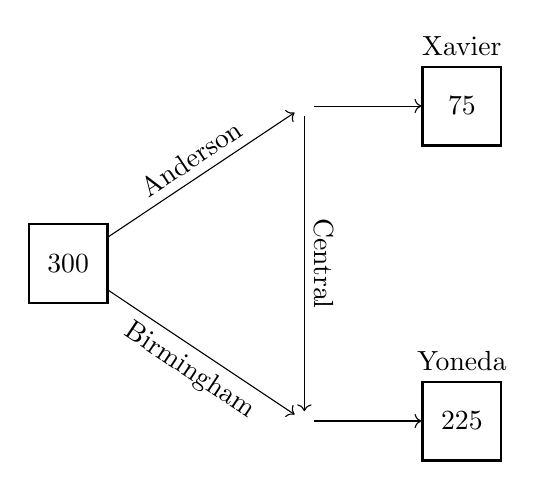
\begin{tikzpicture}
\node (V) at (0,0) [draw,thick,minimum width=1cm,minimum height=1cm] {$300$};

\node (I1) at (3,2) {};
\node (I2) at (3,-2) {};


\draw[->] (V) -- (I1)node[midway,sloped,above]{Anderson};;
\draw[->] (V) -- (I2) node[midway,sloped,below]{Birmingham};
\draw[->] (I1) -- (I2) node[midway,sloped,above]{Central};

\node[label={Xavier}] (X) at (5,2) [draw,thick,minimum width=1cm,minimum height=1cm] {75};

\node[label={Yoneda}] (Y) at (5,-2) [draw,thick,minimum width=1cm,minimum height=1cm] {225};

\draw[->] (I1)--(X);
\draw[->] (I2)--(Y);


\end{tikzpicture}$$

Let $a,b,c$ denote the number of people walking along Anderson, Birmingham and Central.

\begin{enumerate}
    \item Find an expression for the amount of people walking along each street.\\
    
    We first set up our systems of equations.  We first note that all 300 people have to walk either along either Anderson or Birmingham, so $$a+b=300.$$  Next, the 75 at Xavier is the however many people walked down Anderson, and take away whoever veered off onto Central so: $$a-c=75.$$  The 225 people at Yoneda is everyone coming across Birmingham and Central so $$b+c=225.$$  Thus the system is:
    
    \begin{eqnarray*}
    a+b&=&300\\
    a-c&=&75\\
    b+c&=&225,\\
    \end{eqnarray*}
    
    with associated augmented matrix:
    
    $$ \left( \begin{array}{rrr|r}
1 & 1 & 0& 300\\
1 & 0 & -1 & 75\\
0 & 1 & 1 & 225
\end{array}\right).$$
    
So the reduced row echelon form of this is:

    $$ \left( \begin{array}{rrr|r}
1 & 0 & -1 & 75\\
0 & 1 & 1 & 225\\
0 & 0 & 0& 0
\end{array}\right).$$

What this tells us is that there is not a unique solution, as the system associated with this matrix is:

    \begin{eqnarray*}
    a-c&=&75\\
    b+c&=&225,\\
    \end{eqnarray*}

Which is two of the original equations.  So, depending on what $c$ is, this will determine how many people traverse Anderson and Birmingham.

\item If 50 people crossed central, how many people crossed Anderson and Birmingham?\\

So letting $c=50$, we would have:

    \begin{eqnarray*}
    a-c&=&75\\
    a-50&=&75\\
    a&=&125\\
    b+c&=&225\\
    b+50&=&225\\
    b&=&175,
    \end{eqnarray*}
So 125 people across Anderson and 175 across Birmingham.\\

Another way to do this would be to add an equation $c=50$ to our system:

$$ \left( \begin{array}{rrr|r}
1 & 1 & 0& 300\\
1 & 0 & -1 & 75\\
0 & 1 & 1 & 225\\
0 & 0 & 1 & 50
\end{array}\right).$$
    
    Which has reduced row echelon form:
 
 $$ \left( \begin{array}{rrr|r}
1 & 0 & 0 & 125\\
0 & 1 & 0 & 175\\
0 & 0 & 1& 50\\
0 & 0 & 0& 0
\end{array}\right).$$   

That is $a=125, b=125, c=50$ which is our solution above.

\item If 100 people go through Anderson, how many go through Birmingham or Central?\\

We can revisit our linear system from (a):

    \begin{eqnarray*}
    a-c&=&75\\
    100-c&=&75\\
    c&=&25\\
    b+c&=&225\\
    b+25&=&225\\
    b&=&200,
    \end{eqnarray*}
so 200 across Birmingham and 25 across Central.\\

We can also add the linear equation $a=100$:

$$ \left( \begin{array}{rrr|r}
1 & 1 & 0& 300\\
1 & 0 & -1 & 75\\
0 & 1 & 1 & 225\\
1 & 0 & 0 & 100
\end{array}\right)$$

with reduced row echelon form:

$$ \left( \begin{array}{rrr|r}
1 & 0 & 0 & 100\\
0 & 1 & 0 & 200\\
0 & 0 & 1& 25\\
0 & 0 & 0& 0
\end{array}\right).$$  So 100 across Anderson, 200 across Birmingham and 25 across Central.
    
\end{enumerate}



\end{example}

\section{Products and Sums of Matrices}\label{Section:MatrixArithmetic}

In the previous sections, we saw how the entries of matrix may be used to record relationships between two collections of variables.  For example in Example \ref{Example:Vitamin}, the entries in the $3\times 3$ portion of the matrix represents the proportion of vitamins contained by a collection of supplements, with each entry representing a vitamin-supplement pair.  It is natural then, to wonder if we could combine relationships between variables or compose them.  The operations behind these ideas are the sums and products of matrices.

\subsection{Products of Matrices}

We begin with a motivating example:

\begin{example}\label{Example:VitProd}

Recall that in Example \ref{Example:Vitamin} Margo has three supplements: the first contains 20\% vitamin A, 20\% vitamin D and 20\%
vitamin E; the second contains 10\% vitamin A, 30\% vitamin D and 40\% vitamin E; the third contains 50\% vitamin A, 10\% vitamin D and 20\% vitamin E.\\

On Monday she eats 100 mg of supplement 1, 100 mg of supplement 2 and 150 mg of supplement 3.  On Wednesday she eats 150 mg of supplement 1, 50 mg of supplement 2 and 100 mg of supplement 3.  Putting aside that this is an ill advised way to take supplements, how much of each vitamin did she get on each day?\\

We first let $$A= \left( \begin{array}{rrr}
0.2 & 0.1 & 0.5\\
0.2 & 0.3 & 0.1\\
0.2 & 0.4 & 0.2
\end{array}\right)$$

represent the relation between vitamins and supplements, where each row corresponds to vitamins, and each column corresponds to supplements.  So the entry in the second row, second column corresponds to the proportion of supplement 2 which is vitamin D, 30\%.\\

A useful way to conceptualize this matrix is as an arrow or transformation, whose inputs are mg of various supplements, and whose outputs are mg of various vitamins.

$$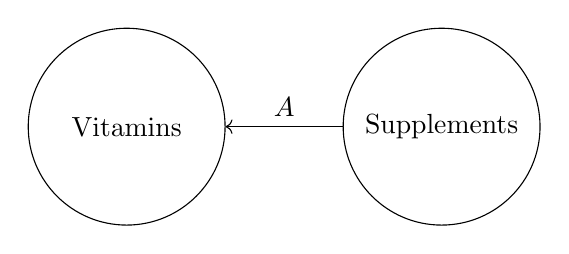
\begin{tikzpicture}
\node(S)[draw,circle,minimum size=2.5cm,inner sep=1pt] at (4,0) {Supplements};
\node(V)[draw,circle,minimum size=2.5cm,inner sep=1pt] at (0,0) {Vitamins};

\draw[->] (S) --node[above]{$A$} (V);

\end{tikzpicture}$$


Next, we record the relationship between days of the week and supplements:

$$B= \left( \begin{array}{rrr}
100 & 150\\
100 & 50\\
150 & 100
\end{array}\right)$$


Where now the rows are quantities of supplements and columns are days of the week.  So the 100 in the third row second column represents the 100mg taken on Wednesday of Supplement 3.  This to may be conceptualized as an arrow or transformation whose inputs are days of the week, and whose outputs are quantities of supplements.

$$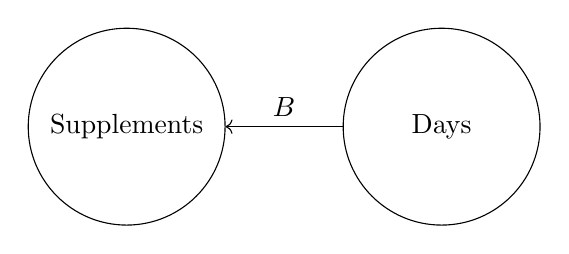
\begin{tikzpicture}
\node(S)[draw,circle,minimum size=2.5cm,inner sep=1pt] at (4,0) {Supplements};
%\node(V)[draw,circle,minimum size=2.5cm,inner sep=1pt] at (0,0) {Vitamins};
\node(D)[draw,circle,minimum size=2.5cm,inner sep=1pt] at (8,0) {Days};

%\draw[->] (S) --node[above]{A} (V);
\draw[->] (D) --node[above]{$B$} (S);

\end{tikzpicture}$$

Our goal now is to establish a relationship between days of the week and quantity of vitamins.

$$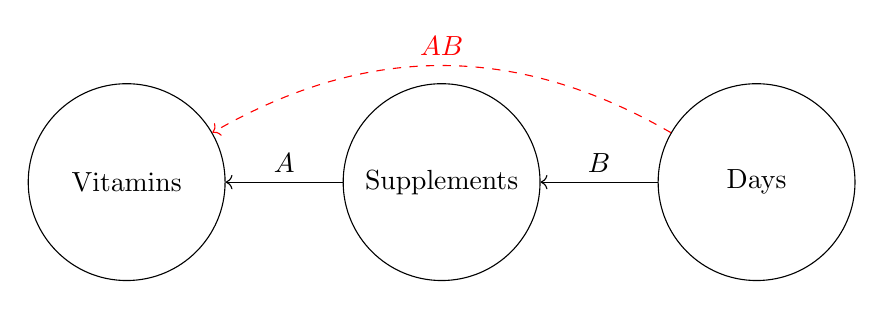
\begin{tikzpicture}
\node(S)[draw,circle,minimum size=2.5cm,inner sep=1pt] at (4,0) {Supplements};
\node(V)[draw,circle,minimum size=2.5cm,inner sep=1pt] at (0,0) {Vitamins};
\node(D)[draw,circle,minimum size=2.5cm,inner sep=1pt] at (8,0) {Days};

\draw[->] (S) --node[above]{$A$} (V);
\draw[->] (D) --node[above]{$B$} (S);

\draw [->, dashed, red] (D) to [out=150,in=30] node[above]{$AB$} (V);


\end{tikzpicture}$$

So, how much Vitamin A does Margo get on Monday?  She took \textcolor{blue}{100} mg of Supplement 1, of which \textcolor{red}{20\%} is Vitamin A, \textcolor{blue}{100} mg of Supplement 2, of which \textcolor{red}{10\%} is Vitamin A, and \textcolor{blue}{150} mg of Supplement 1, of which \textcolor{red}{50\%} is Vitamin A:

$$\left( \begin{array}{rrr}
\textcolor{red}{0.2} & \textcolor{red}{0.1} & \textcolor{red}{0.5}\\
0.2 & 0.3 & 0.1\\
0.2 & 0.4 & 0.2
\end{array}\right)\left( \begin{array}{rrr}
\textcolor{blue}{100} & 150\\
\textcolor{blue}{100} & 50\\
\textcolor{blue}{150} & 100
\end{array}\right)=\left( \begin{array}{cr}
\textcolor{red}{0.2}\cdot\textcolor{blue}{100}+\textcolor{red}{0.1}\cdot\textcolor{blue}{100}+\textcolor{red}{0.5}\cdot\textcolor{blue}{150} & ? \\
? & ? \\
? & ? 
\end{array}\right)=\left( \begin{array}{cr}
105 & ? \\
? & ? \\
? & ? 
\end{array}\right).$$

So on Monday, Margo got 105 mg of vitamin A.  What about the amount of vitamin D she received on Wednesday?  She took \textcolor{blue}{150} mg of Supplement 1, of which \textcolor{red}{20\%} is Vitamin D, \textcolor{blue}{50} mg of Supplement 2, of which \textcolor{red}{30\%} is Vitamin D, and \textcolor{blue}{100} mg of Supplement 1, of which \textcolor{red}{10\%} is Vitamin A:

\begin{eqnarray*}
\left( \begin{array}{rrr}
0.2 & 0.1 & 0.5\\
\textcolor{red}{0.2} & \textcolor{red}{0.3} & \textcolor{red}{0.1}\\
0.2 & 0.4 & 0.2
\end{array}\right)\left( \begin{array}{rrr}
100 & \textcolor{blue}{150}\\
100 & \textcolor{blue}{50}\\
150 & \textcolor{blue}{100}
\end{array}\right)&=&\left( \begin{array}{cr}
105 & ? \\
? & \textcolor{red}{0.2}\cdot\textcolor{blue}{150}+\textcolor{red}{0.3}\cdot\textcolor{blue}{50}+\textcolor{red}{0.1}\cdot\textcolor{blue}{100} \\
? & ? 
\end{array}\right)\\
&=&\left( \begin{array}{cr}
105 & ? \\
? & 55 \\
? & ? 
\end{array}\right).
\end{eqnarray*}

So Margo got 55 mg of Vitamin D on Wednesday.  Following this line of thinking, we obtain matrix:

$$\left( \begin{array}{rrr}
{0.2} & {0.1} & {0.5}\\
0.2 & 0.3 & 0.1\\
0.2 & 0.4 & 0.2
\end{array}\right)\left( \begin{array}{rrr}
{100} & 150\\
{100} & 50\\
{150} & 100
\end{array}\right)=\left( \begin{array}{cr}
105 & 85 \\
65 & 55 \\
90 & 70 
\end{array}\right).$$

This matrix records how much of each vitamin Margo had per day, where vitamins are rows and days are columns.  So on Monday, she got 90 mg of Vitamin E, and on Wednesday, she got 85 mg of Vitamin A.

\end{example}

So with this illustrative example in mind, we can define matrix multiplication.

\begin{definition}\label{Defn:MatrixProd}
For any matrix $M$, let $(M)_{ij}=m_{ij}$ denote the entry in the $i$th row and $j$th column.   Then, given a $m\times n$ matrix $A$ and a $n\times k$ matrix $B$, we define $AB$ the product of $A$ and $B$ to be a $m\times k$ matrix where:

$$(AB)_{ij}=\begin{pmatrix}\textcolor{red}{a_{i1}} & \textcolor{red}{a_{i2}} & \cdots & \textcolor{red}{a_{in}}\end{pmatrix}\begin{pmatrix}\textcolor{blue}{b_{1j}} \\ \textcolor{blue}{b_{2j}} \\ \vdots \\ \textcolor{blue}{b_{nj}}\end{pmatrix}=\begin{pmatrix}\textcolor{red}{a_{i1}}\textcolor{blue}{b_{1j}}+\textcolor{red}{a_{i2}}\textcolor{blue}{b_{2j}}+\cdots+\textcolor{red}{a_{in}}\textcolor{blue}{b_{nj}} \end{pmatrix}$$

\end{definition}

\textbf{Note that the number of columns of $A$ and the number of rows of $B$ must be the same.}  Recall Example \ref{Example:VitProd}, the outputs of $B$ corresponded to the rows, and the inputs of $A$ corresponded to it's columns, so these had to match up.  This number is also the $n$ is Definition \ref{Defn:MatrixProd}.


\begin{example}\label{Example:MoreMatrixProducts}
Let $$A=\begin{pmatrix}
1 & 2 & 3\\ 4 & 5 & 6
\end{pmatrix}, B=\begin{pmatrix}
0.2 & 0.4 \\ 0.5 & 0.6 \\ 0.1 & 0.8
\end{pmatrix}, C=\begin{pmatrix}
10 \\ 20 \\ 15
\end{pmatrix}.$$
Find:

\begin{enumerate}
    \item $AB$.
    \begin{eqnarray*}
    AB=\begin{pmatrix}
1 & 2 & 3\\ 4 & 5 & 6
\end{pmatrix}\begin{pmatrix}
0.2 & 0.4 \\ 0.5 & 0.6 \\ 0.1 & 0.8
\end{pmatrix}&=&\begin{pmatrix}
1\cdot0.2+2\cdot0.5+3\cdot0.1 & 1\cdot0.4+2\cdot0.6+3\cdot0.8\\
4\cdot0.2+5\cdot0.5+6\cdot0.1 & 4\cdot0.4+5\cdot0.6+6\cdot0.8 
\end{pmatrix}\\
&=&\begin{pmatrix}
1.5 & 4 \\ 3.9  &  9.4
\end{pmatrix}
    \end{eqnarray*}
    
    
    
    \item $BA$.
    \begin{eqnarray*}
    BA=\begin{pmatrix}
0.2 & 0.4 \\ 0.5 & 0.6 \\ 0.1 & 0.8
\end{pmatrix}\begin{pmatrix}
1 & 2 & 3\\ 4 & 5 & 6
\end{pmatrix}&=&\begin{pmatrix}
0.2\cdot1+ 0.4\cdot 4 & 0.2\cdot2+ 0.4\cdot 5 & 0.2\cdot3+ 0.4\cdot6\\
0.5\cdot1+ 0.6\cdot 4 & 0.5\cdot2+ 0.6\cdot 5 & 0.5\cdot3+ 0.6\cdot6\\
0.1\cdot1+ 0.8\cdot 4 & 0.1\cdot2+ 0.8\cdot 5 & 0.1\cdot3+ 0.8\cdot6\\
\end{pmatrix}\\
&=&\begin{pmatrix}
1.8 & 2.4 & 3 \\ 2.9  &  4 & 5.1 \\ 3.3 & 4.2 & 5.1
\end{pmatrix}
    \end{eqnarray*}    
    
    \item $AC$.
    \begin{eqnarray*}
    AC=\begin{pmatrix}
1 & 2 & 3\\ 4 & 5 & 6
\end{pmatrix}\begin{pmatrix}
10\\20\\15
\end{pmatrix}&=&\begin{pmatrix}
1\cdot10+2\cdot20+3\cdot15 \\ 4\cdot10+5\cdot20+6\cdot15
\end{pmatrix}\\
&=&\begin{pmatrix}
95 \\ 230
\end{pmatrix}
    \end{eqnarray*}
    
    
    
    \item $CA$.
    
    Notice that if we try to take the product $CA$:
    \begin{eqnarray*}
    CA=\begin{pmatrix}
10\\20\\15
\end{pmatrix}\begin{pmatrix}
1 & 2 & 3\\ 4 & 5 & 6
\end{pmatrix}&=&\begin{pmatrix}
10\cdot1+?\cdot4 & 10\cdot2+?\cdot5 & 10\cdot3+?\cdot6 \\ 20\cdot1+?\cdot4 & 20\cdot2+?\cdot5 & 20\cdot3+?\cdot6\\15\cdot1+?\cdot4 & 15\cdot2+?\cdot5 & 15\cdot3+?\cdot6
\end{pmatrix}
    \end{eqnarray*}
Since the number of columns of the first matrix do not match with the number of rows of the second matrix, the product is not defined.    
    
    \item $BC$.
    
    Since $B$ has 2 columns and $C$ has 3 rows, these values do not match and this product is not defined.
    \item $CB$.
    
    Since $C$ has 1 column and $B$ has 2 rows, these values do not match and this product is not defined.
\end{enumerate}


\end{example}

Something we should observe here is that, unlike products of real numbers, products of matrices are \textbf{NOT} commutative.  In Example \ref{Example:MoreMatrixProducts}, $AB\neq BA$, and $AC$ was defined whereas $CA$ was not.

Another way matrix products deviate from real number products is that the product of matrices whose entries aren't 0 can result in a matrix whose entries are all 0.

\begin{example}
Let $$A=\begin{pmatrix}1&2\\2&4 \end{pmatrix}, B=\begin{pmatrix}2&6\\-1&-3 \end{pmatrix}.$$

Notice that:

\begin{eqnarray*}
AB=\begin{pmatrix}1&2\\2&4 \end{pmatrix}\begin{pmatrix}2&6\\-1&-3 \end{pmatrix}&=&\begin{pmatrix}
1\cdot 2+2\cdot(-1) & 1\cdot 6+2\cdot(-3)\\ 2\cdot 2+4\cdot(-1)&2\cdot 6 +4\cdot(-3)
\end{pmatrix}\\
&=&\begin{pmatrix}
0 & 0 \\ 0 & 0
\end{pmatrix}.
\end{eqnarray*}
Although neither $A$ nor $B$ have 0 entries, their product is an all 0 matrix.  Also notice that this does not mean $BA$ is an all 0 matrix.

\begin{eqnarray*}
BA=\begin{pmatrix}2&6\\-1&-3 \end{pmatrix}\begin{pmatrix}1&2\\2&4 \end{pmatrix}&=&\begin{pmatrix}
2\cdot 1+6\cdot2 & 2\cdot 2+6\cdot4\\ (-1)\cdot 1+(-3)\cdot2&(-1)\cdot 2 +(-3)\cdot4
\end{pmatrix}\\
&=&\begin{pmatrix}
14 & 28 \\ -7 & -14
\end{pmatrix}.
\end{eqnarray*}

\end{example}






\subsection{Sums of Matrices}

Matrix sums are much more straight forward than their products.  Two Matrices need to have the same dimensions in order to be summed, and the sum is just the sum of the entries, so:

$$\begin{pmatrix} a & b \\ c & d \end{pmatrix}+ \begin{pmatrix} w & x \\ y & z \end{pmatrix}=\begin{pmatrix} a+w & b+x \\ c+y & d+z \end{pmatrix}$$


\begin{example}
Company $B$ gets in on this action and will give 2 dollars to each charity for each student who attends.  NOW given $F$ female and $M$ male students, how much money will go to Elderly and the Homeless?

\begin{eqnarray*}
\begin{pmatrix} 0.8 & 0.5 & 0 \\ 0.2 & 0.5 & 1 \end{pmatrix} \left( \begin{pmatrix} 2 & 1 \\ 1 & 2 \\ 2 & 2\end{pmatrix} + \begin{pmatrix} 2 & 2 \\ 2 & 2 \\ 2 & 2\end{pmatrix}   \right)\begin{pmatrix} F\\M \end{pmatrix}&=&\begin{pmatrix} 0.8 & 0.5 & 0 \\ 0.2 & 0.5 & 1 \end{pmatrix} \begin{pmatrix} 4 & 3 \\ 3 & 4 \\ 4 & 4\end{pmatrix} \begin{pmatrix} F\\M \end{pmatrix}\\
&=&\begin{pmatrix} 4.7 & 4.4 \\ 7.3 &  6.6 \end{pmatrix}\begin{pmatrix} F\\M \end{pmatrix}\\
&=&\begin{pmatrix} 4.7F+4.4M\\ 7.3F+6.6M \end{pmatrix}\\
\end{eqnarray*}
So \$$4.7 F+4.4M$ for Elderly and $\$7.3 F+6.6M$ for Homeless.
\end{example}

\section{Computation using Sage}\label{Section:MatrixSage}

As usual, this seems like it should be much easier using technology.  Let's suppose $A=\begin{pmatrix} 1 & 2 \\ 3 & 4\end{pmatrix}, B=\begin{pmatrix} 5 & 6 \\ 7 & 8\end{pmatrix}$.  Verify that:

\begin{eqnarray*}
A+B&=&\begin{pmatrix} 6 & 8 \\ 10 & 12\end{pmatrix}\\
AB&=&\begin{pmatrix} 19 & 22 \\ 43 & 50\end{pmatrix}\\
BA&=&\begin{pmatrix} 23 & 34 \\ 31 & 46\end{pmatrix}
\end{eqnarray*}


\url{https://sagecell.sagemath.org/?z=eJxztM1NLCnKrNAIDNRRiI421DGK1Yk21jGJjdXk5XJClTTVMQNKmutYgCULijLzSjQctZ0QbC0E20nLURMAu6IZgA==&lang=sage}


\end{document}
